\begin{figure}[ht]
	\centering
	\subfigure[bayes]{
		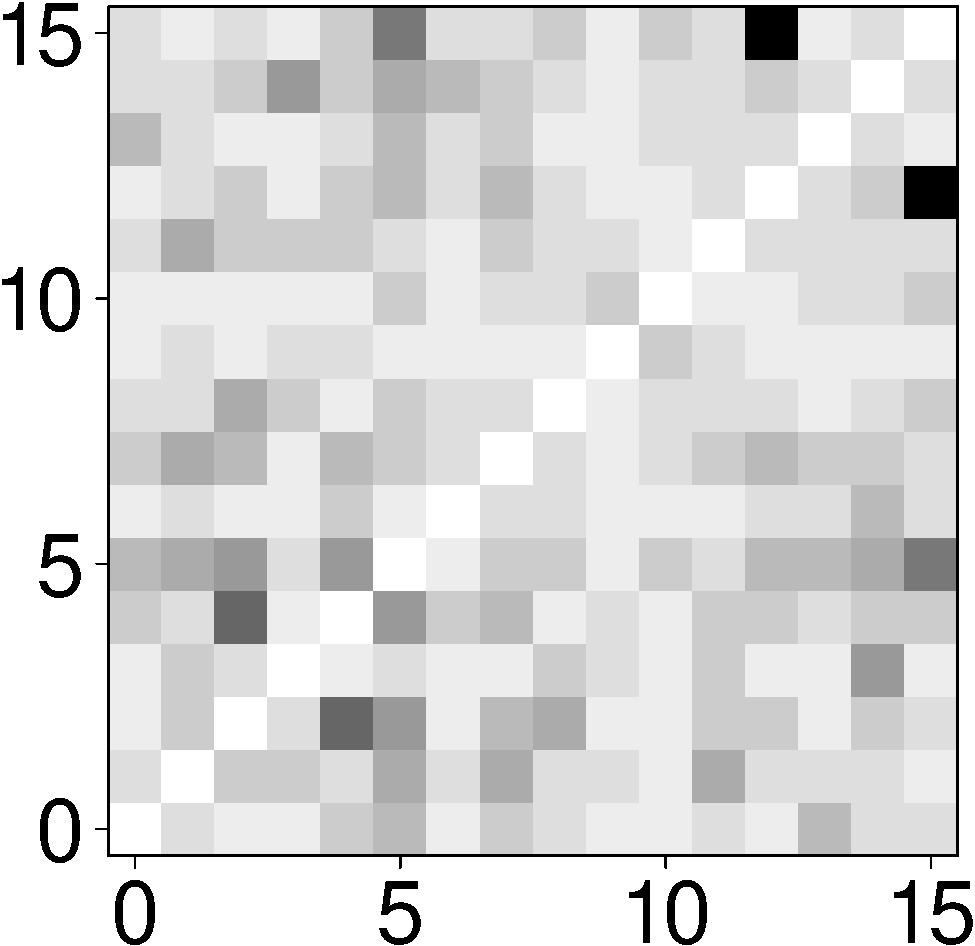
\includegraphics[width=\oneFPage\textwidth]{figures/mechanism/matrices/opteron/bayes_16.pdf}
	}
	\subfigure[genome]{
		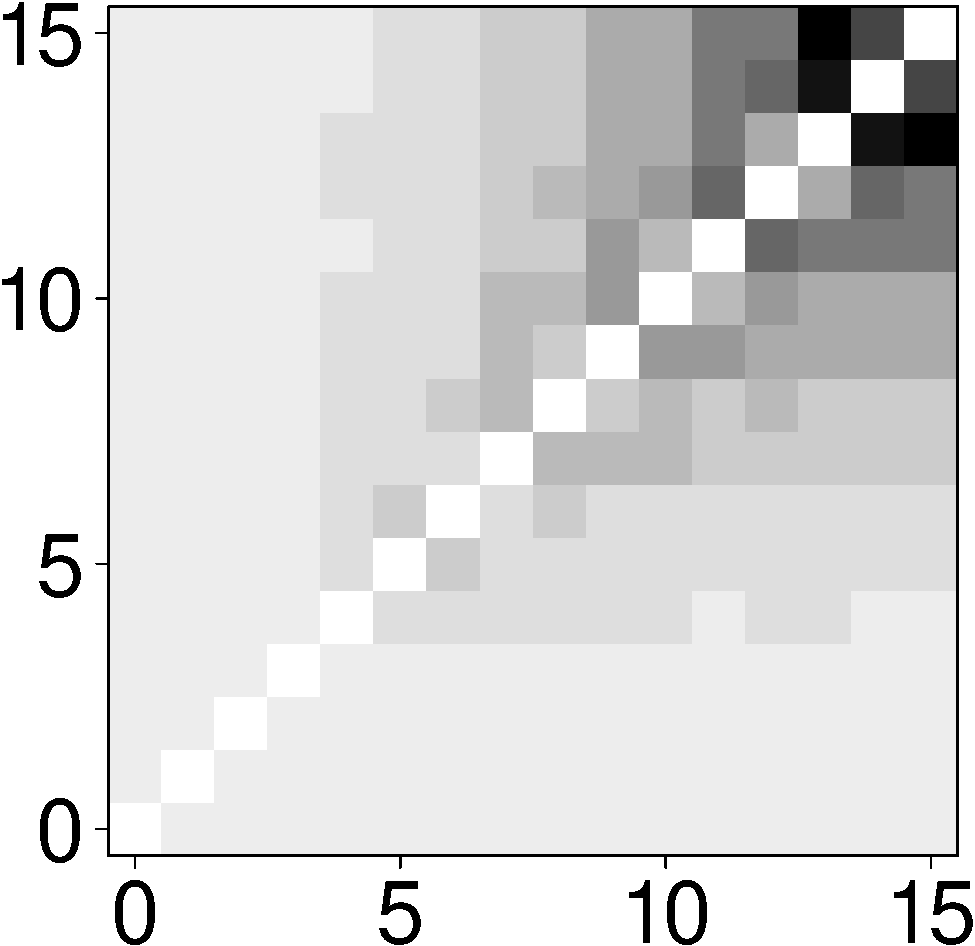
\includegraphics[width=\oneFPage\textwidth]{figures/mechanism/matrices/opteron/genome_16.pdf}
	}
	\subfigure[intruder]{
		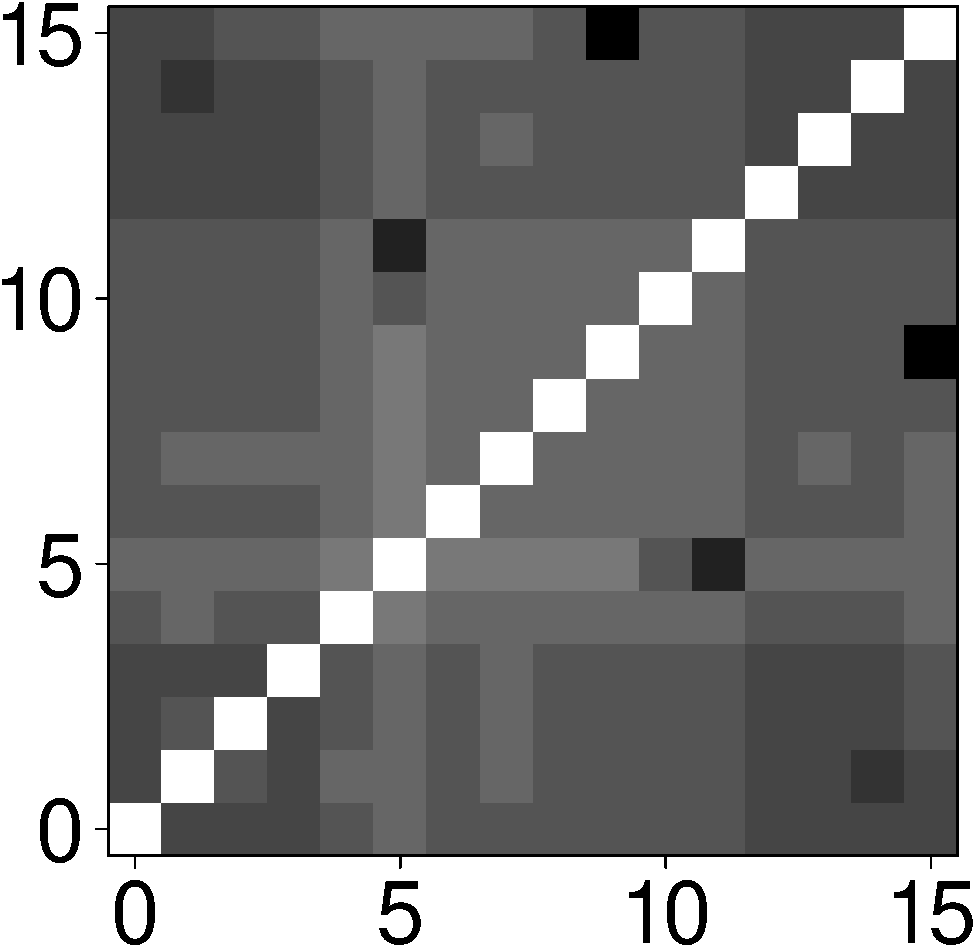
\includegraphics[width=\oneFPage\textwidth]{figures/mechanism/matrices/opteron/intruder_16.pdf}
	}
	\subfigure[kmeans]{
		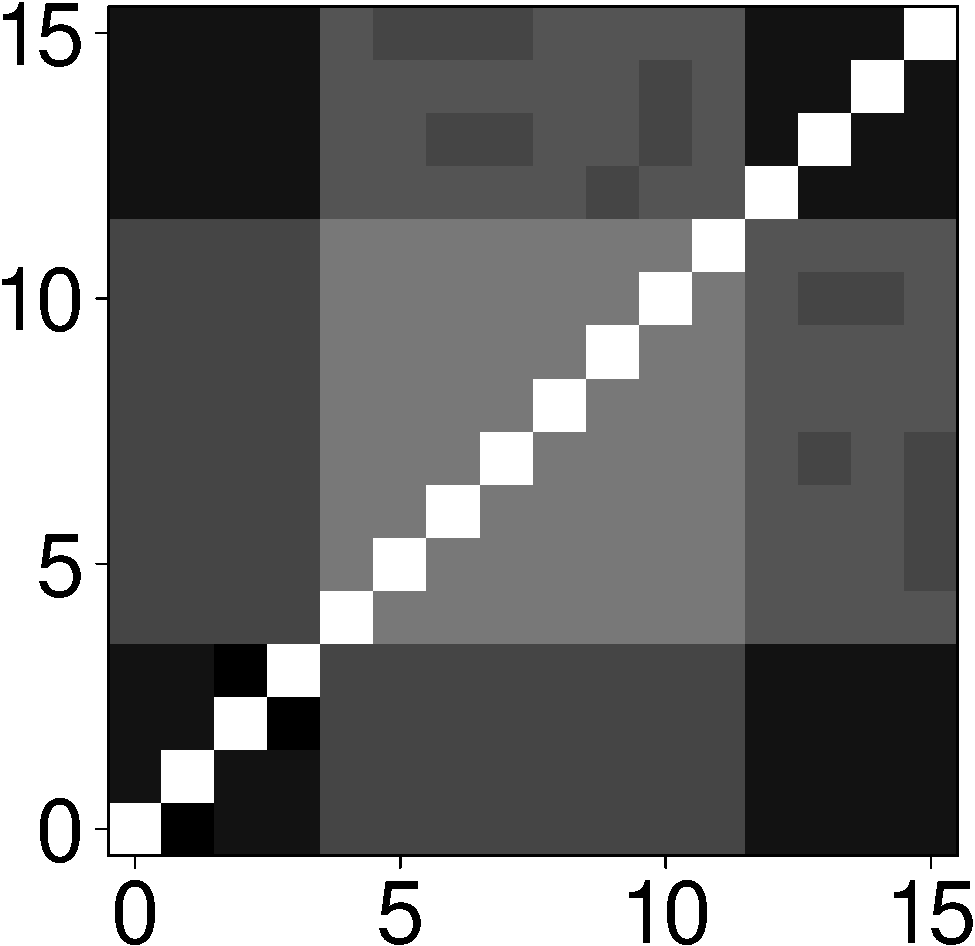
\includegraphics[width=\oneFPage\textwidth]{figures/mechanism/matrices/opteron/kmeans_16.pdf}
	}
	\subfigure[labyrinth]{
		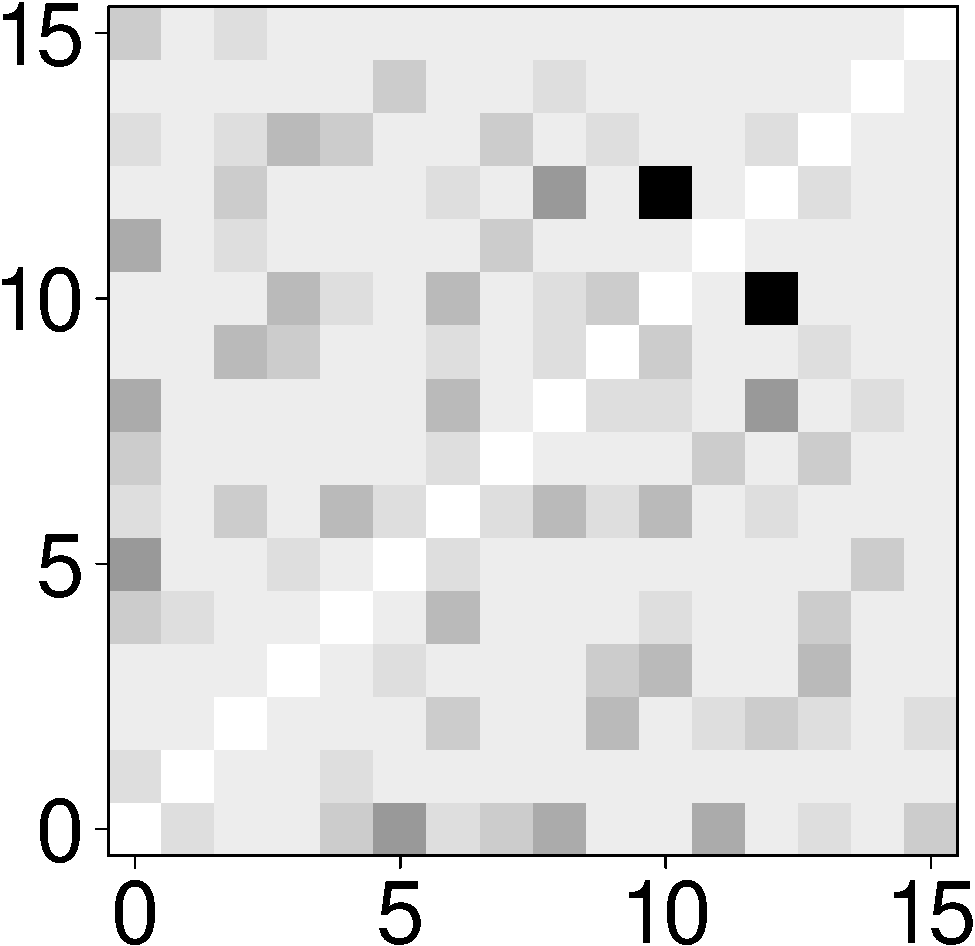
\includegraphics[width=\oneFPage\textwidth]{figures/mechanism/matrices/opteron/labyrinth_16.pdf}
	}
	\\
	\subfigure[ssca2]{
		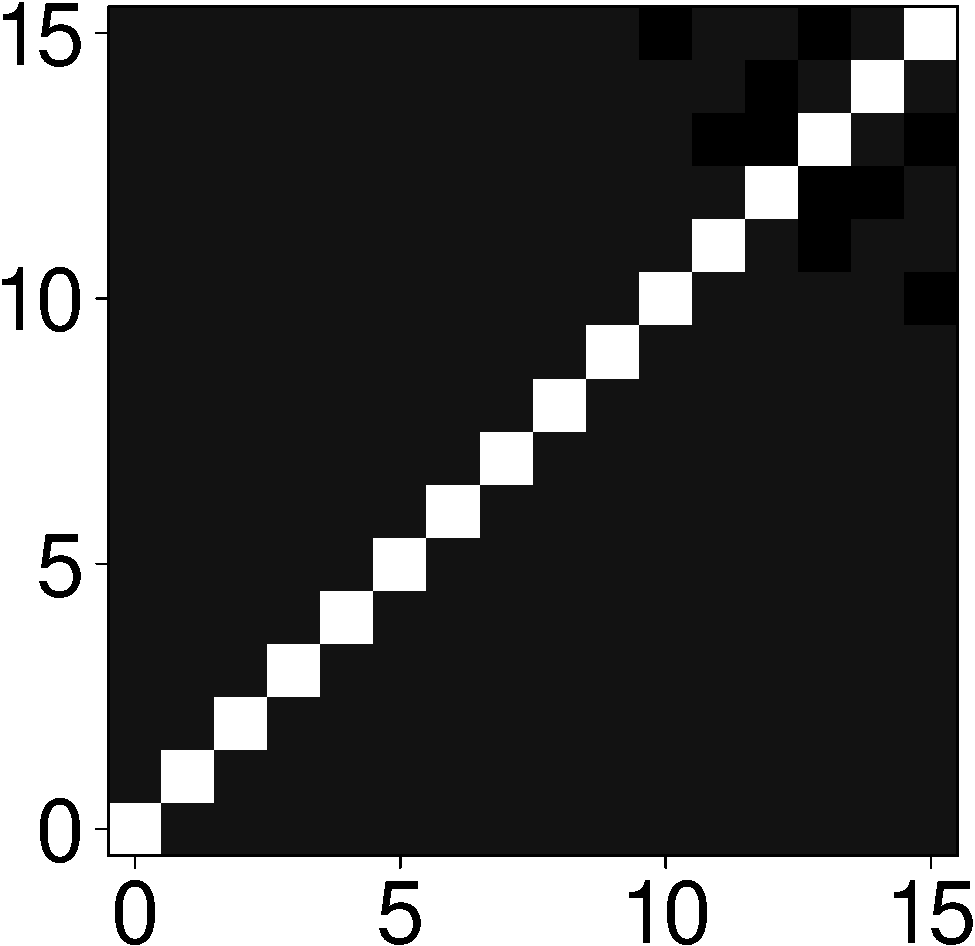
\includegraphics[width=\oneFPage\textwidth]{figures/mechanism/matrices/opteron/ssca2_16.pdf}
	}
	\subfigure[vacation]{
		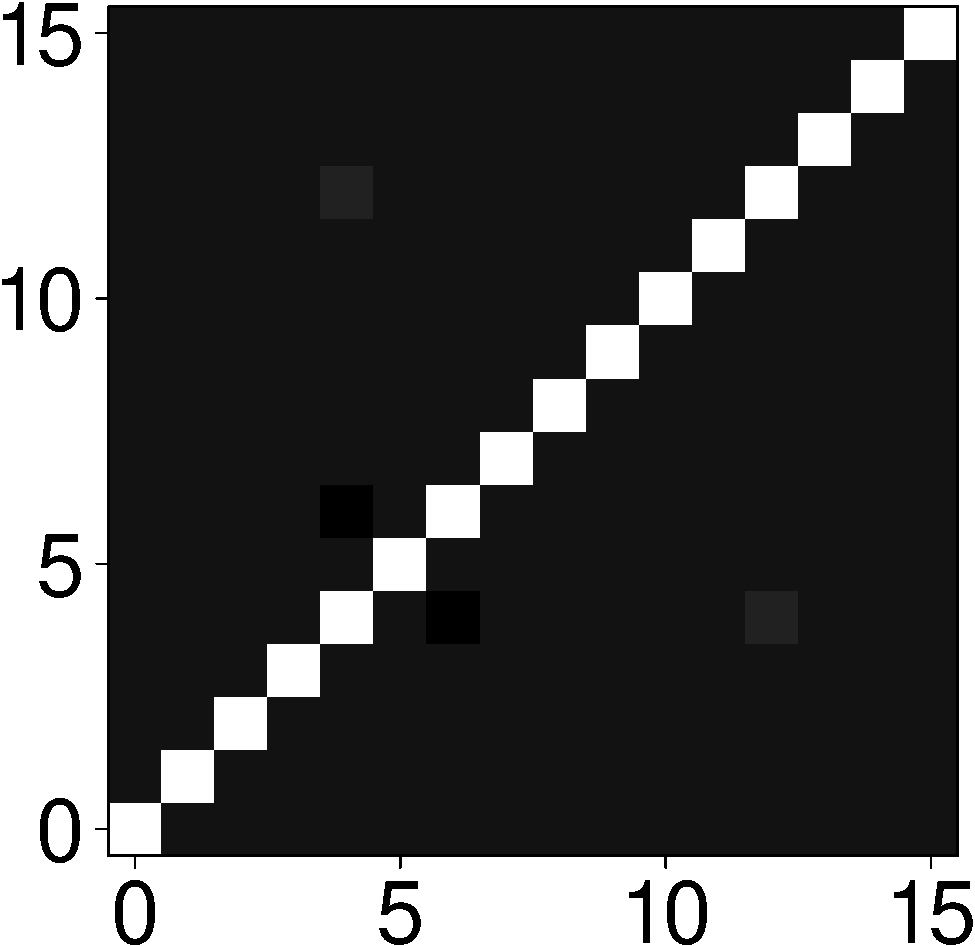
\includegraphics[width=\oneFPage\textwidth]{figures/mechanism/matrices/opteron/vacation_16.pdf}
	}
	\subfigure[yada]{
		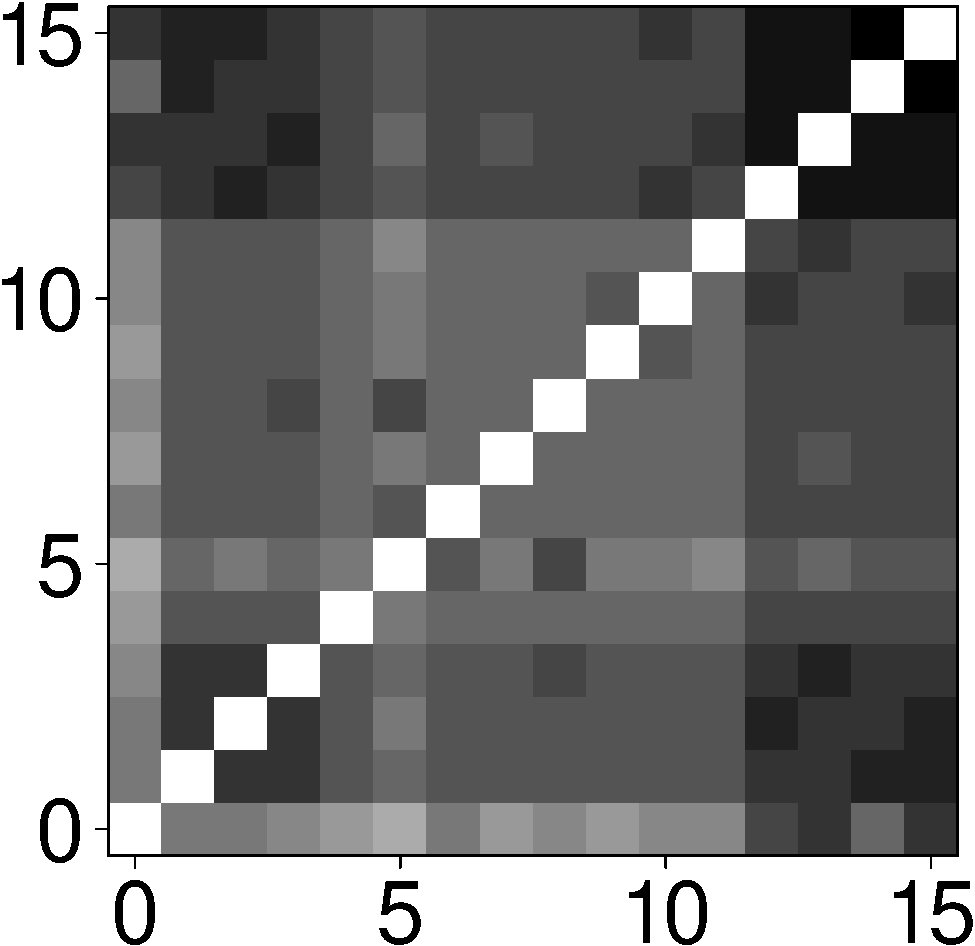
\includegraphics[width=\oneFPage\textwidth]{figures/mechanism/matrices/opteron/yada_16.pdf}
	}
	\subfigure[redblacktree]{
		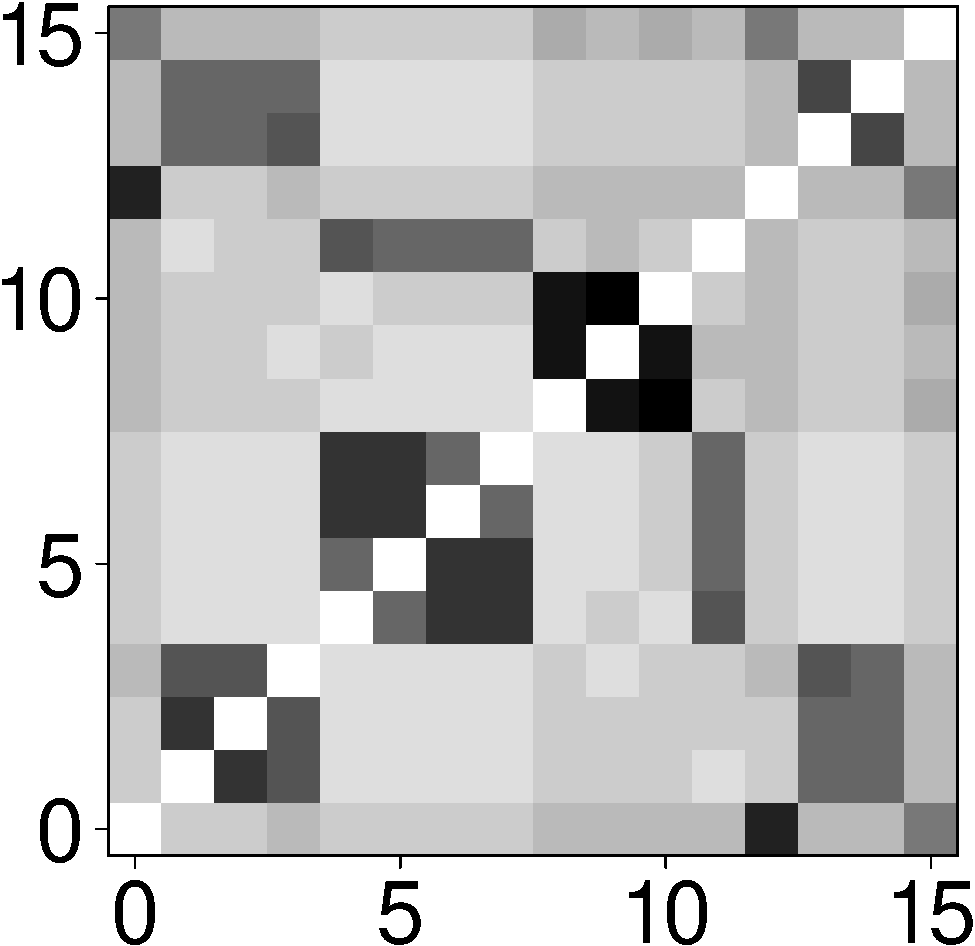
\includegraphics[width=\oneFPage\textwidth]{figures/mechanism/matrices/opteron/redblacktree_16.pdf}
	}
	\subfigure[hashmap]{
		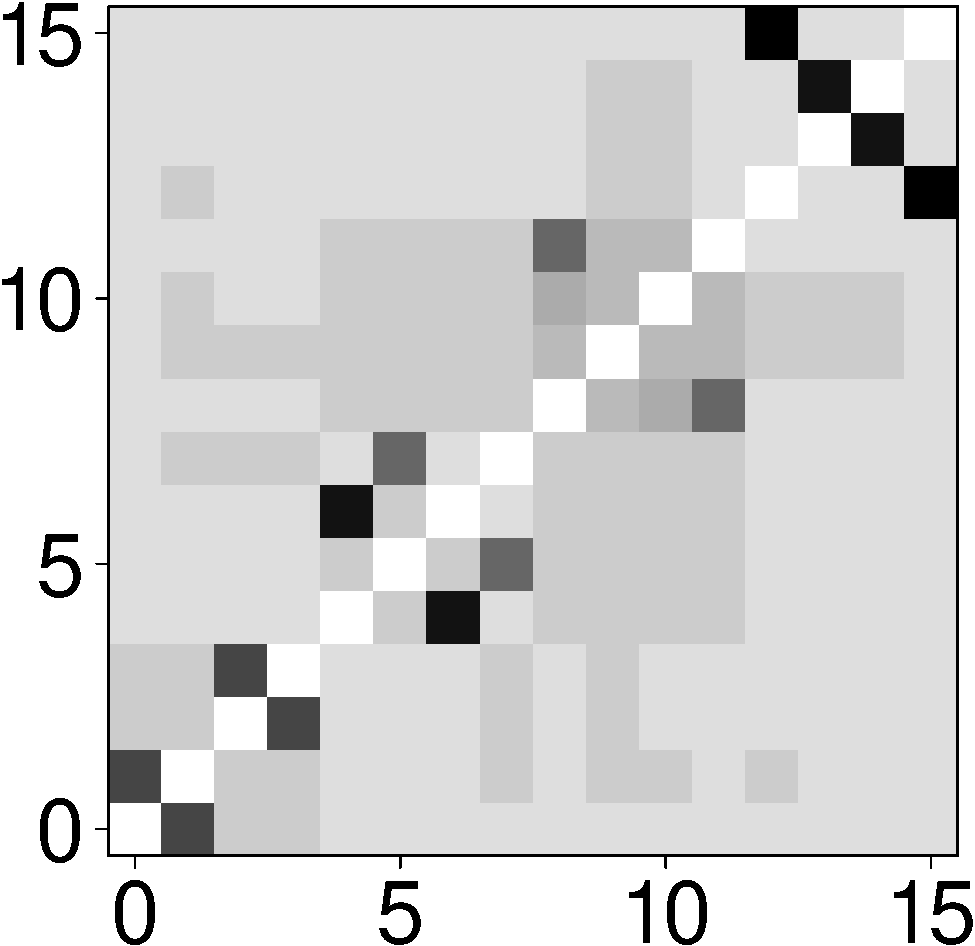
\includegraphics[width=\oneFPage\textwidth]{figures/mechanism/matrices/opteron/hashmap_16.pdf}
	}
	\caption{Communication matrices - 16 threads.}
	\label{fig:commMatrOpt16}
\end{figure}

\begin{figure}[!bt]
	\centering
	\subfigure[bayes]{
		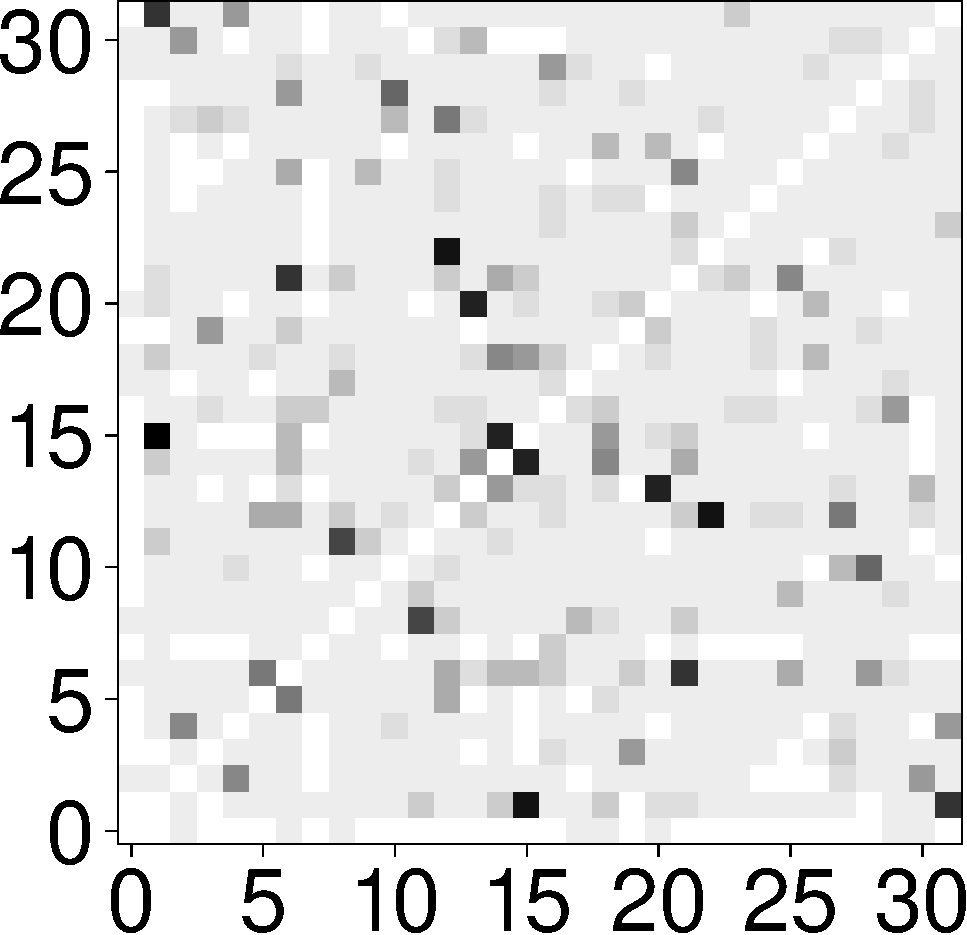
\includegraphics[width=\oneFPage\textwidth]{figures/mechanism/matrices/xeon/bayes_32.pdf}
	}
	\subfigure[genome]{
		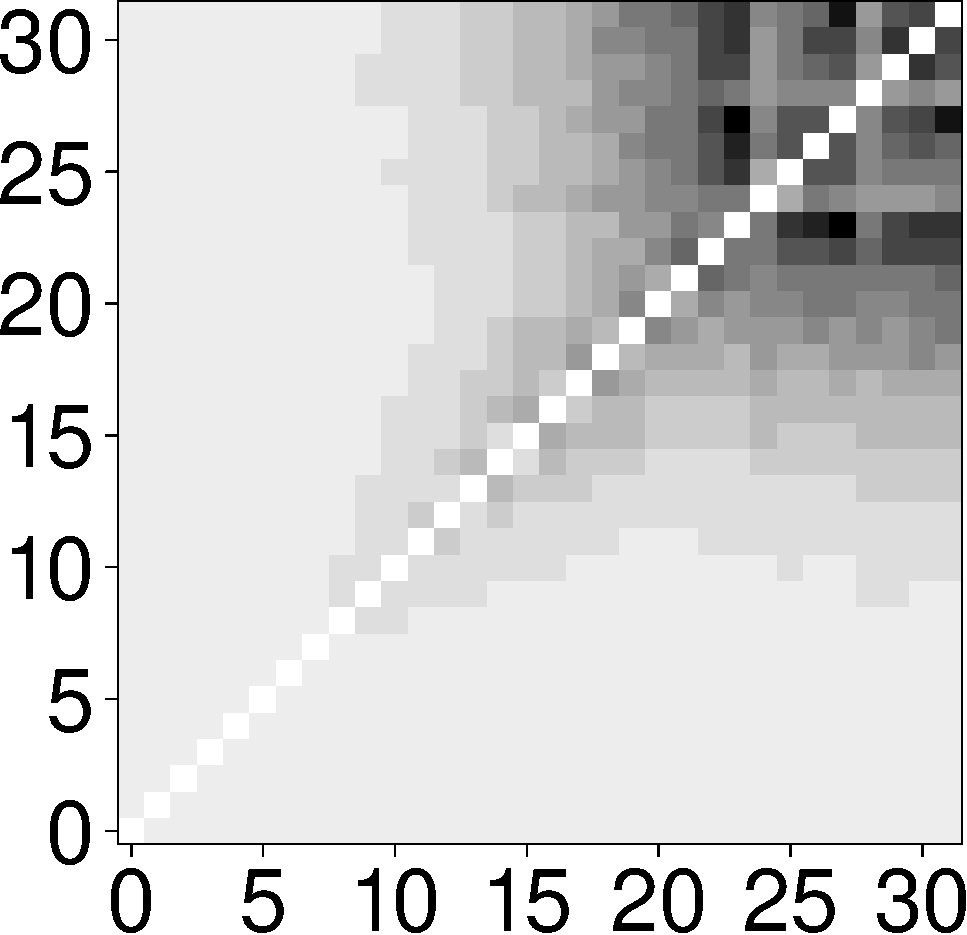
\includegraphics[width=\oneFPage\textwidth]{figures/mechanism/matrices/xeon/genome_32.pdf}
	}
	\subfigure[intruder]{
		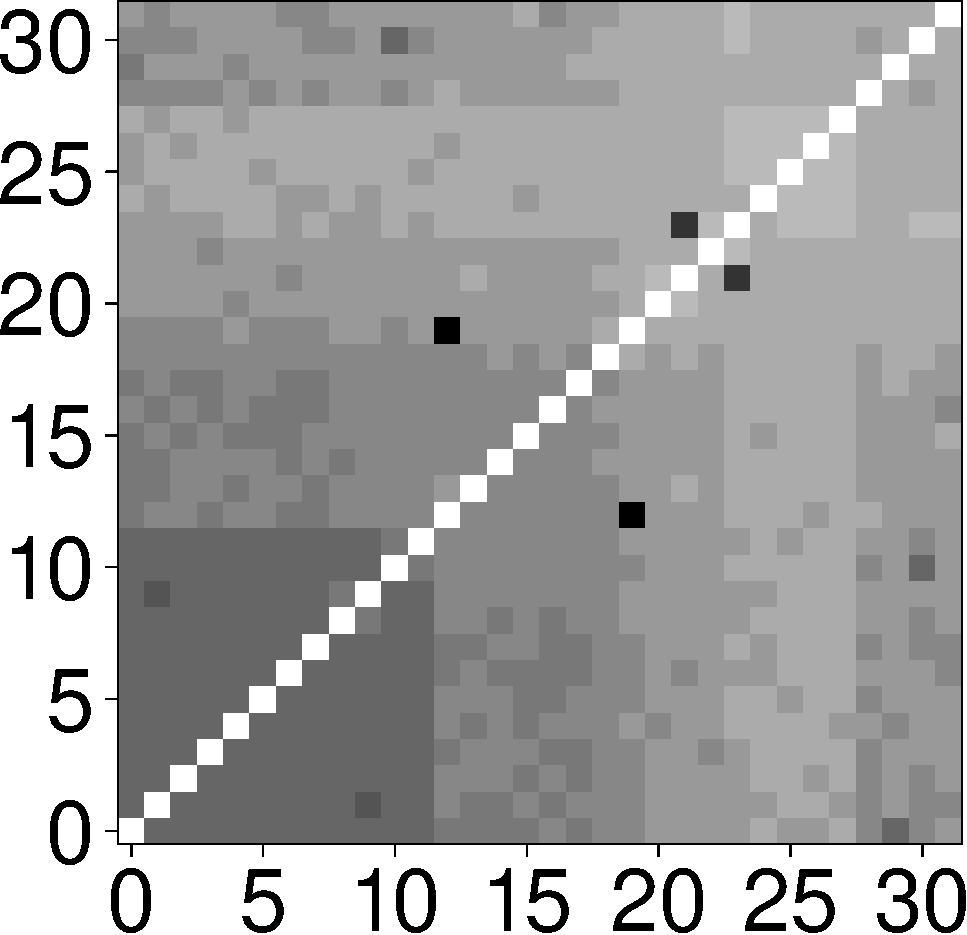
\includegraphics[width=\oneFPage\textwidth]{figures/mechanism/matrices/xeon/intruder_32.pdf}
	}
	\subfigure[kmeans]{
		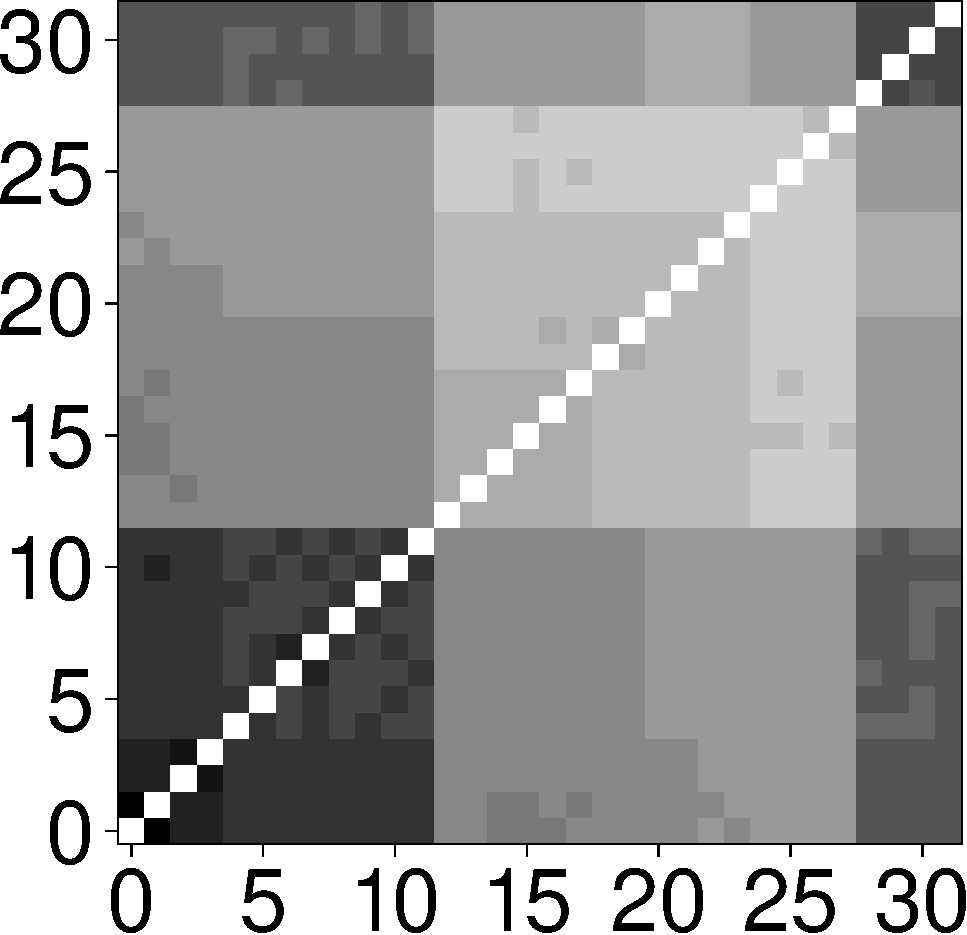
\includegraphics[width=\oneFPage\textwidth]{figures/mechanism/matrices/xeon/kmeans_32.pdf}
	}
	\subfigure[labyrinth]{
		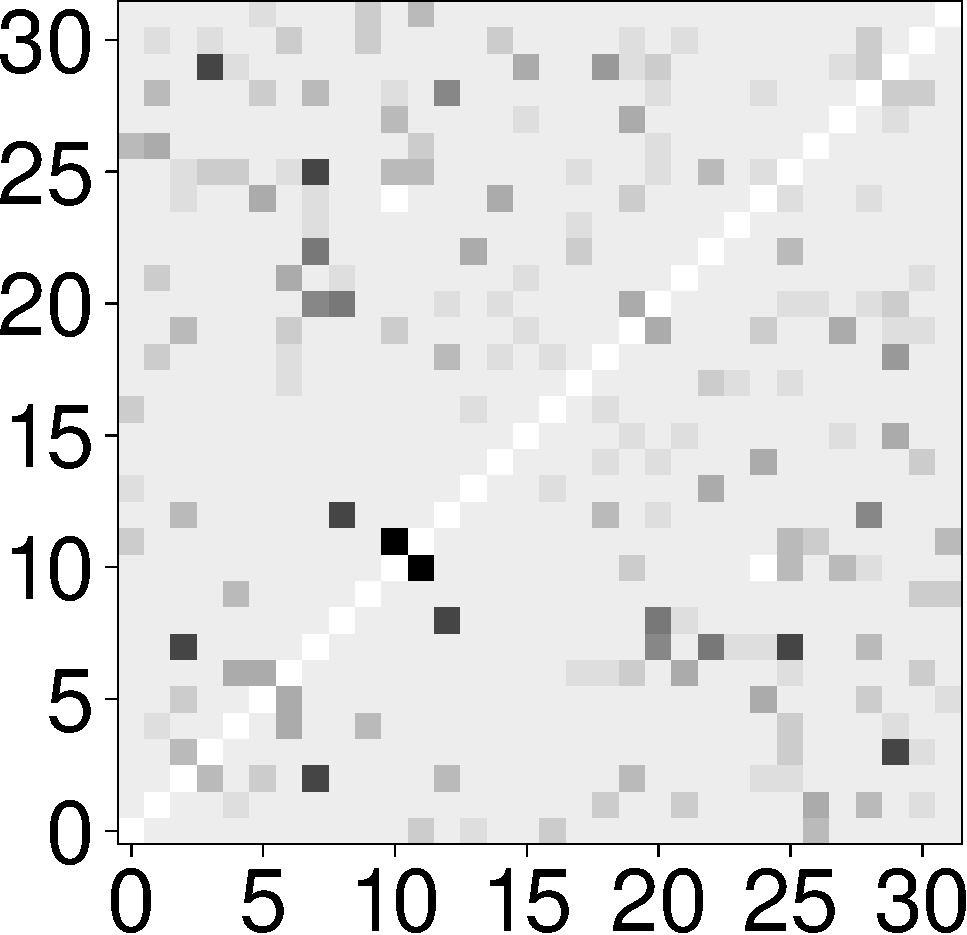
\includegraphics[width=\oneFPage\textwidth]{figures/mechanism/matrices/xeon/labyrinth_32.pdf}
	}
\\
	\subfigure[ssca2]{
		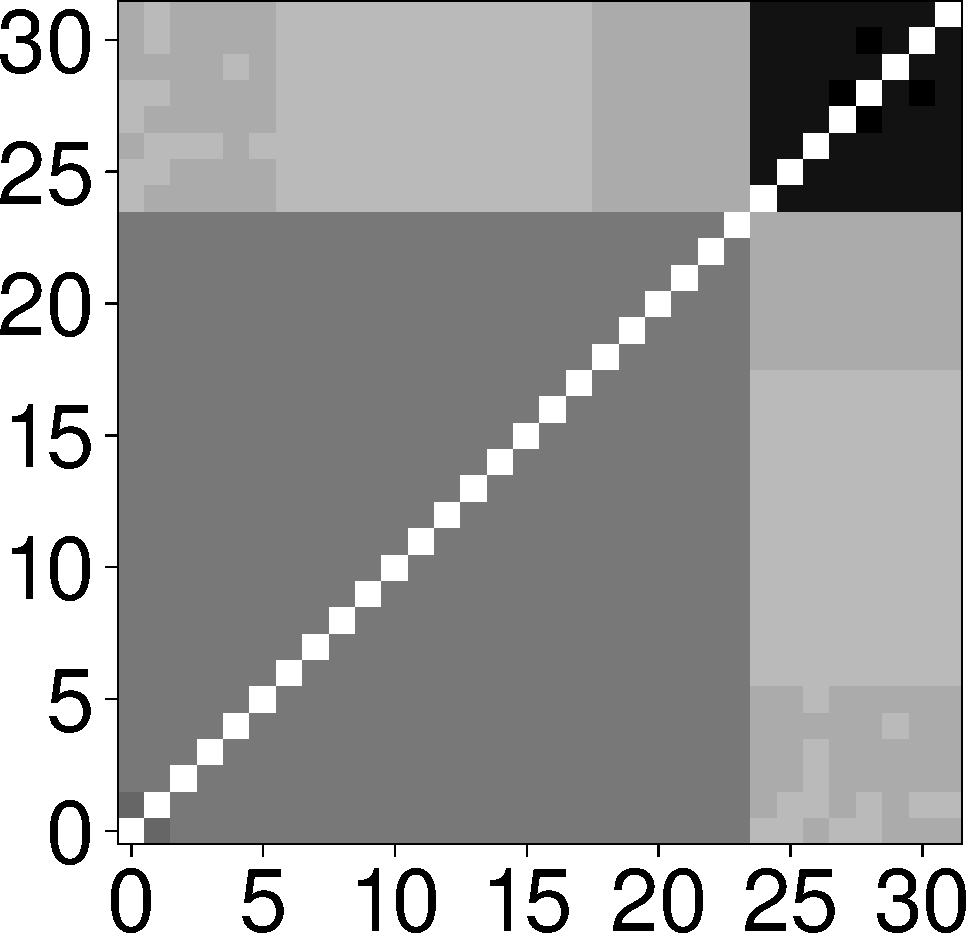
\includegraphics[width=\oneFPage\textwidth]{figures/mechanism/matrices/xeon/ssca2_32.pdf}
	}
	\subfigure[vacation]{
		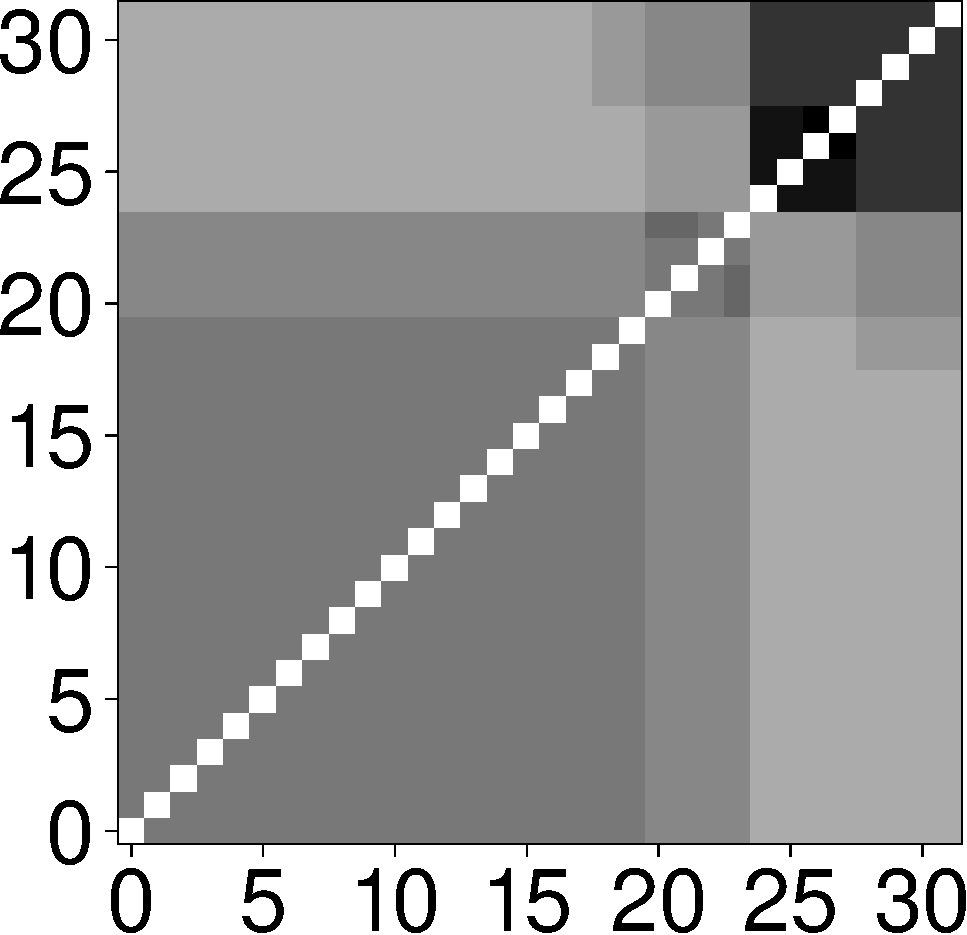
\includegraphics[width=\oneFPage\textwidth]{figures/mechanism/matrices/xeon/vacation_32.pdf}
	}
	\subfigure[yada]{
		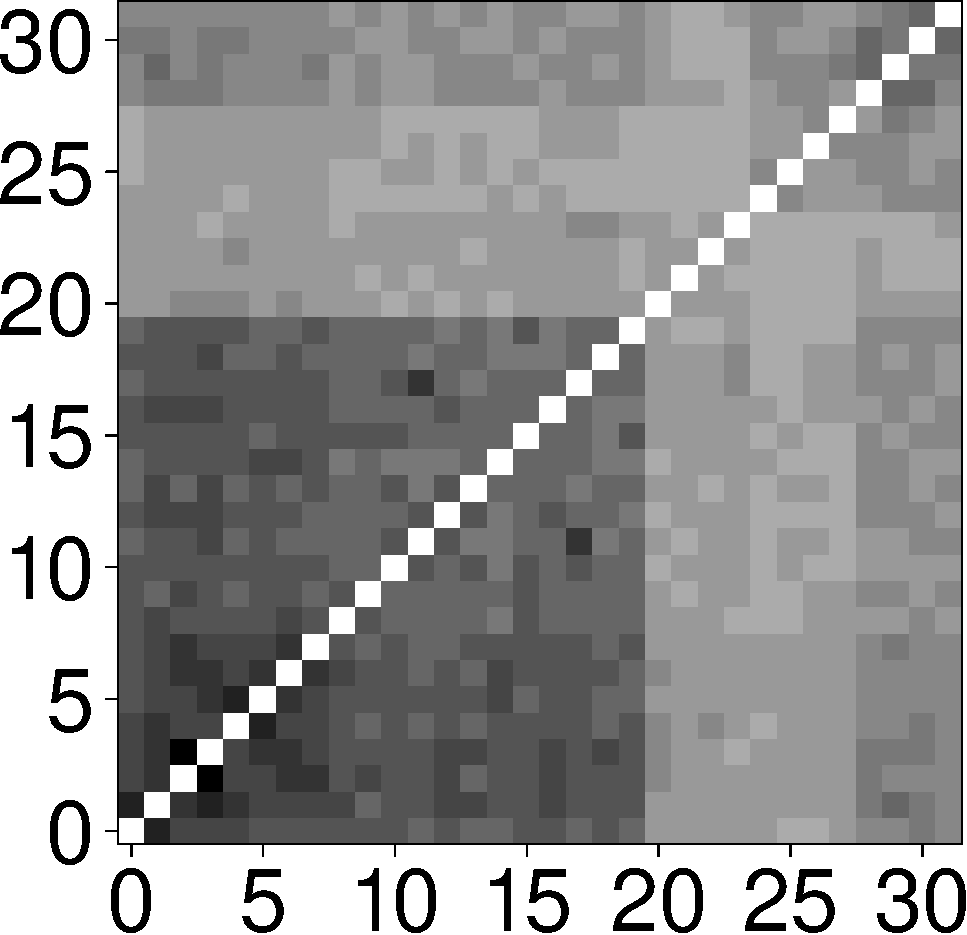
\includegraphics[width=\oneFPage\textwidth]{figures/mechanism/matrices/xeon/yada_32.pdf}
	}
	\subfigure[redblacktree]{
		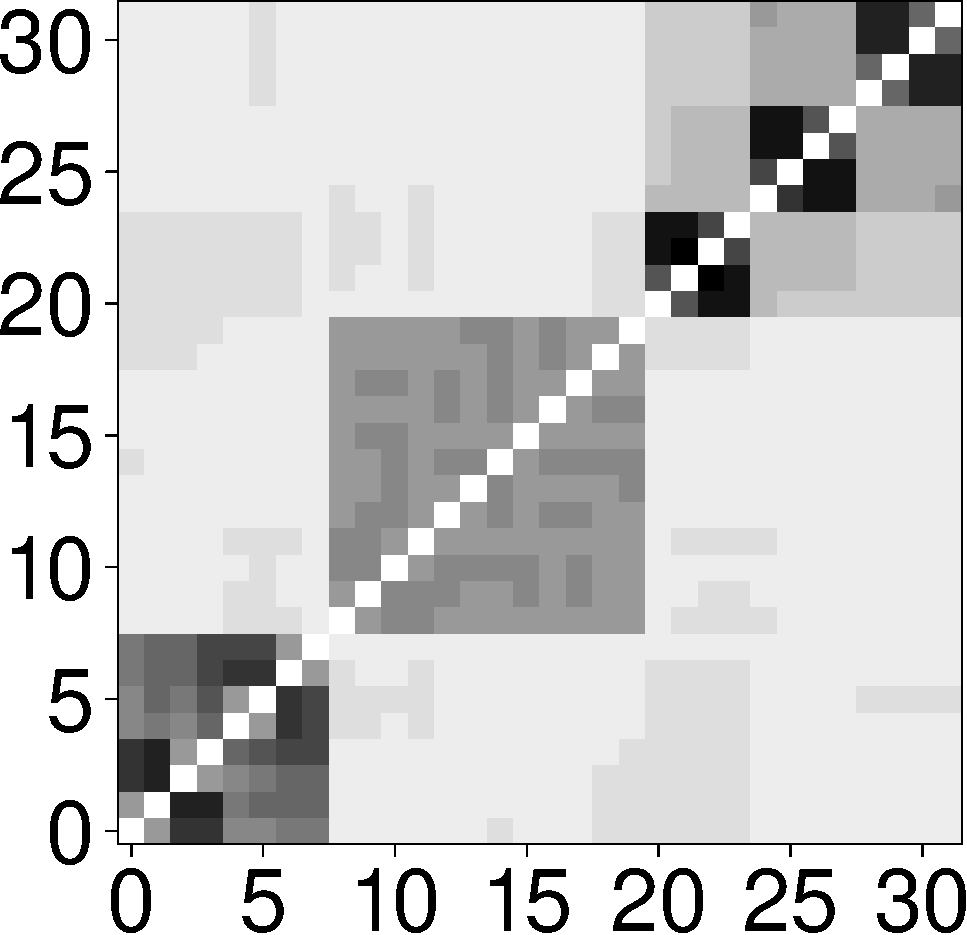
\includegraphics[width=\oneFPage\textwidth]{figures/mechanism/matrices/xeon/redblacktree_32.pdf}
	}
	\subfigure[hashmap]{
		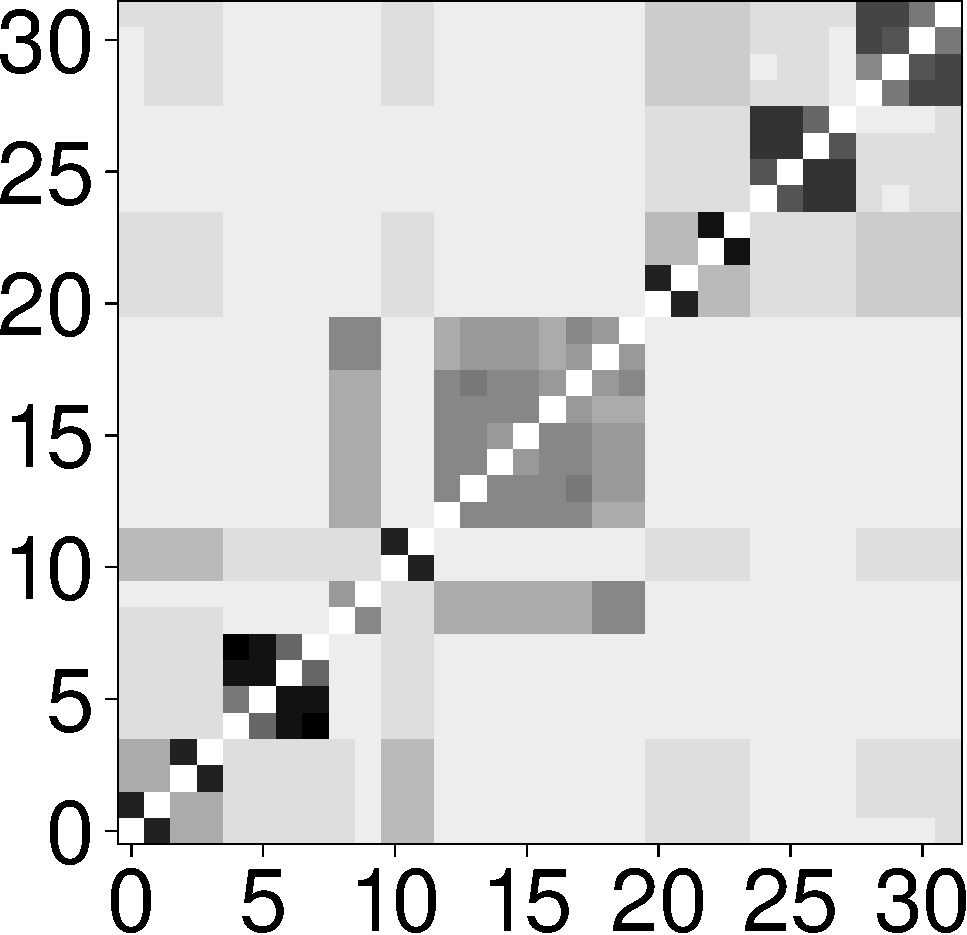
\includegraphics[width=\oneFPage\textwidth]{figures/mechanism/matrices/xeon/hashmap_32.pdf}
	}
	\caption{Communication matrices - 32 threads.}
\end{figure}

%%%%%%%%%%%%%%%%%%%

\begin{figure}[!bt]
	\centering
	\subfigure[bayes]{
		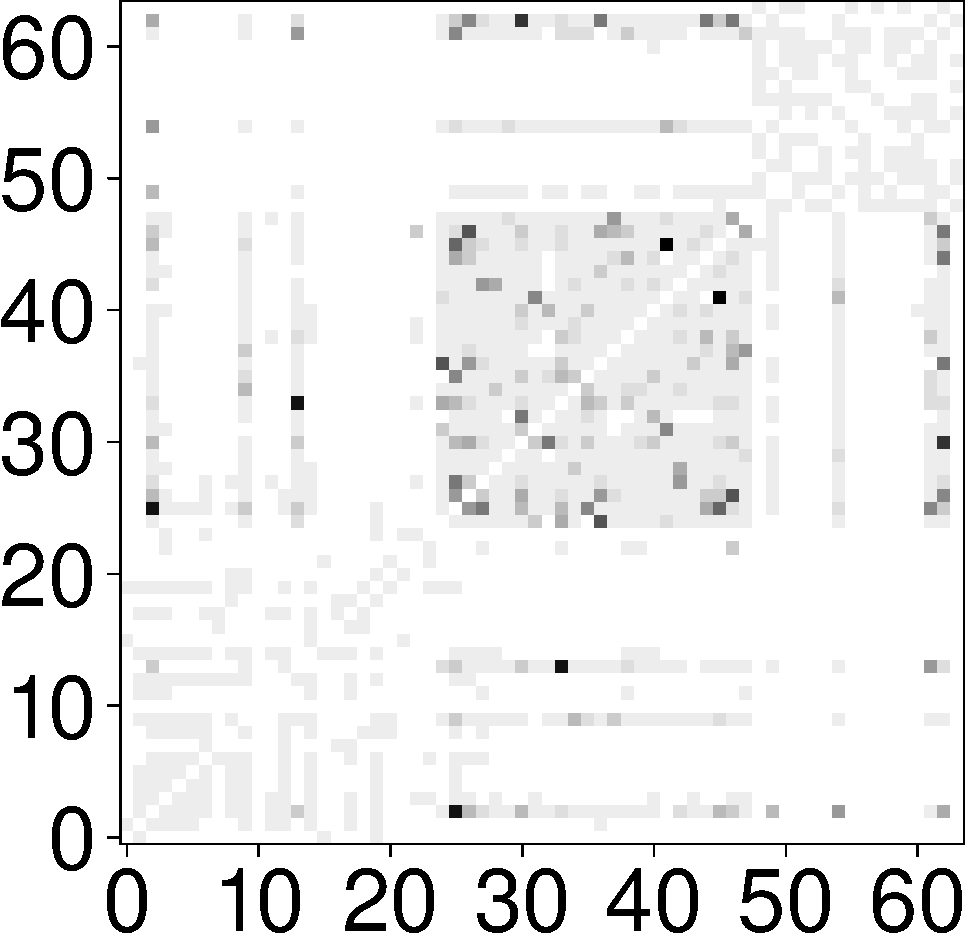
\includegraphics[width=\oneFPage\textwidth]{figures/mechanism/matrices/xeon/bayes_64.pdf}
	}
	\subfigure[genome]{
		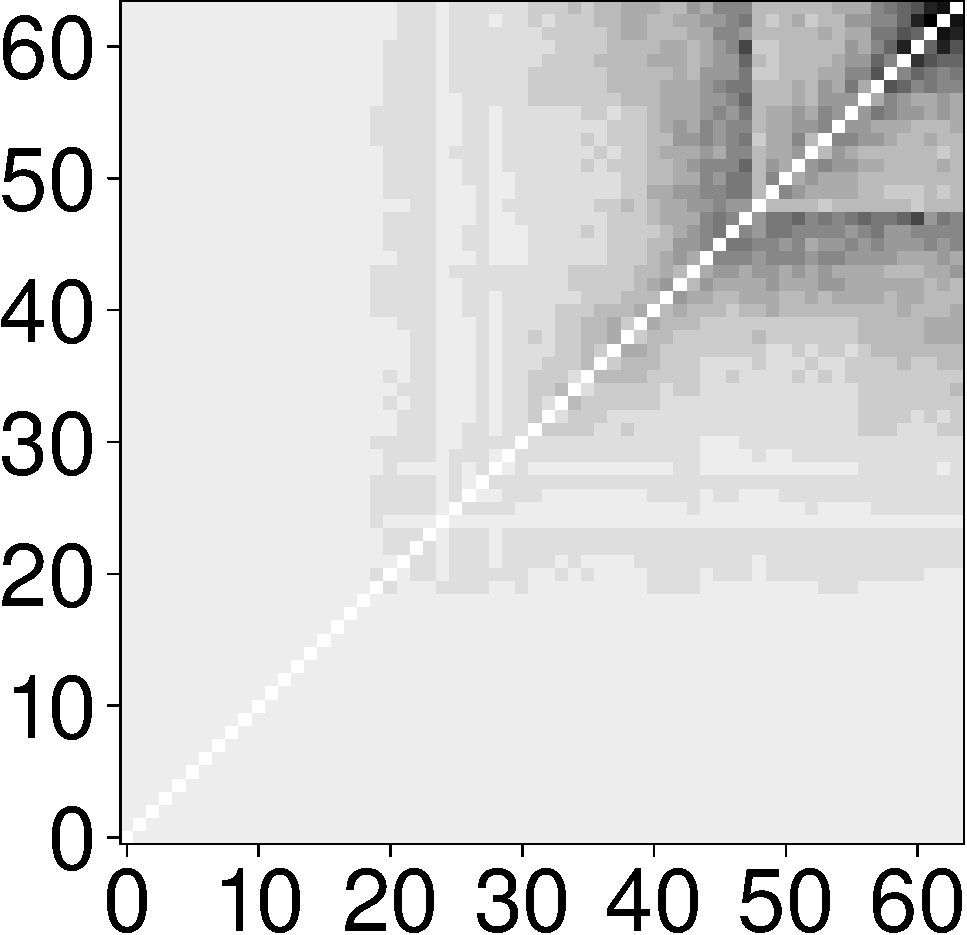
\includegraphics[width=\oneFPage\textwidth]{figures/mechanism/matrices/xeon/genome_64.pdf}
	}
	\subfigure[intruder]{
		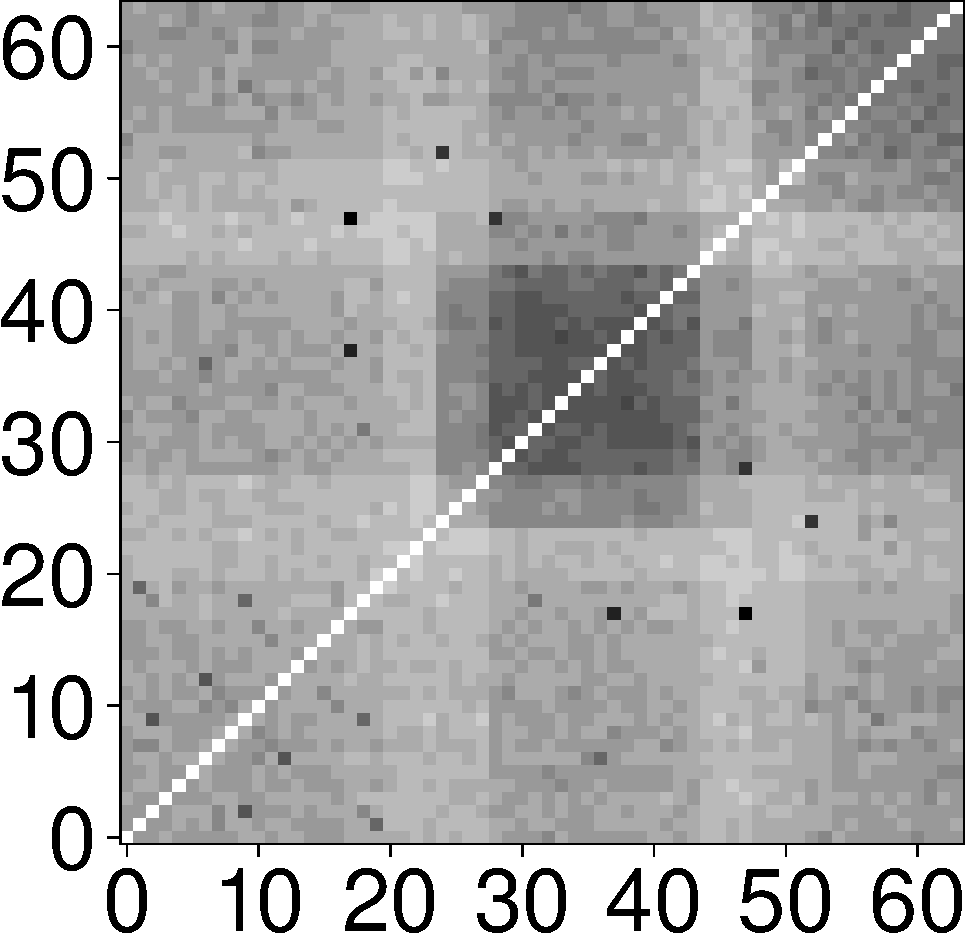
\includegraphics[width=\oneFPage\textwidth]{figures/mechanism/matrices/xeon/intruder_64.pdf}
	}
	\subfigure[kmeans]{
		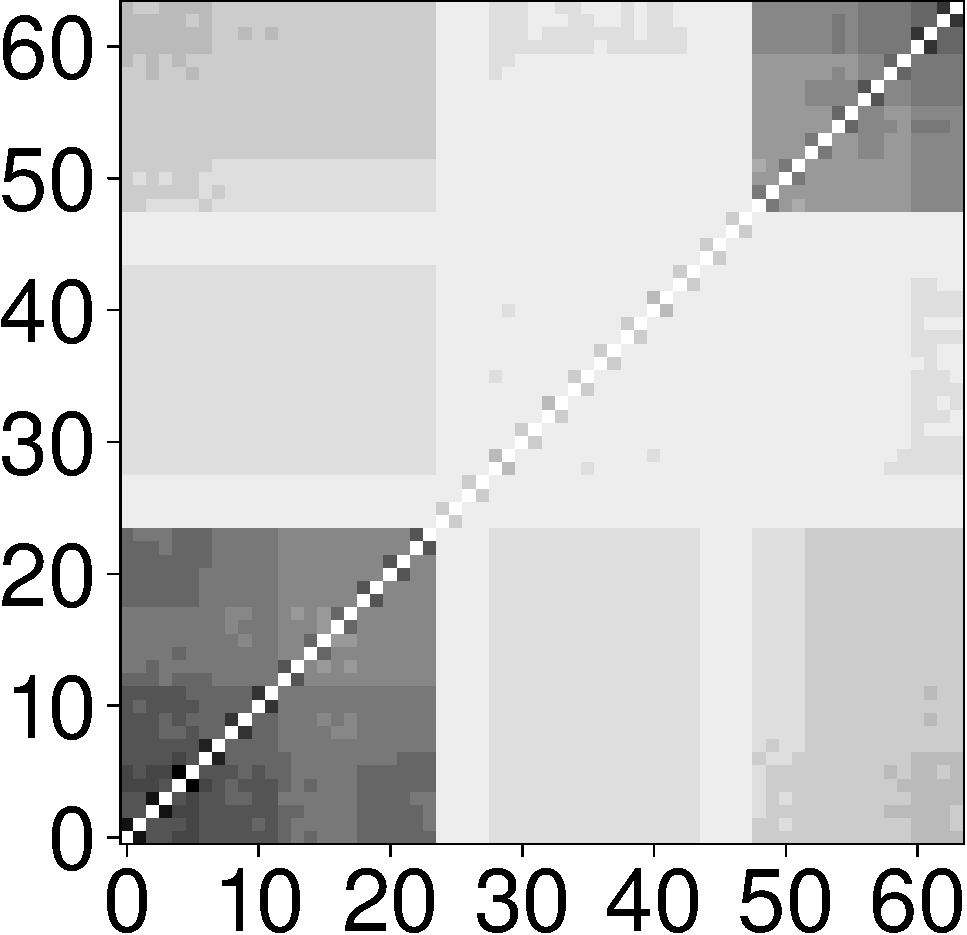
\includegraphics[width=\oneFPage\textwidth]{figures/mechanism/matrices/xeon/kmeans_64.pdf}
	}
	\subfigure[labyrinth]{
		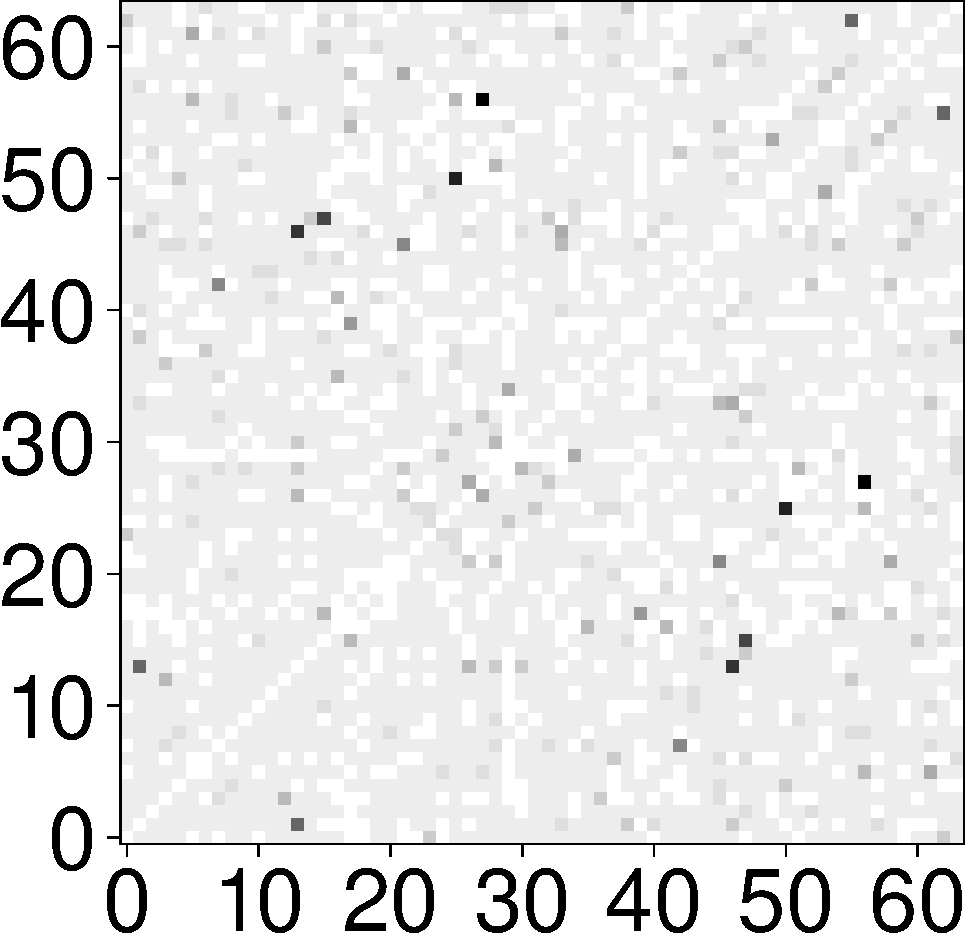
\includegraphics[width=\oneFPage\textwidth]{figures/mechanism/matrices/xeon/labyrinth_64.pdf}
	}
	\\
	\subfigure[ssca2]{
		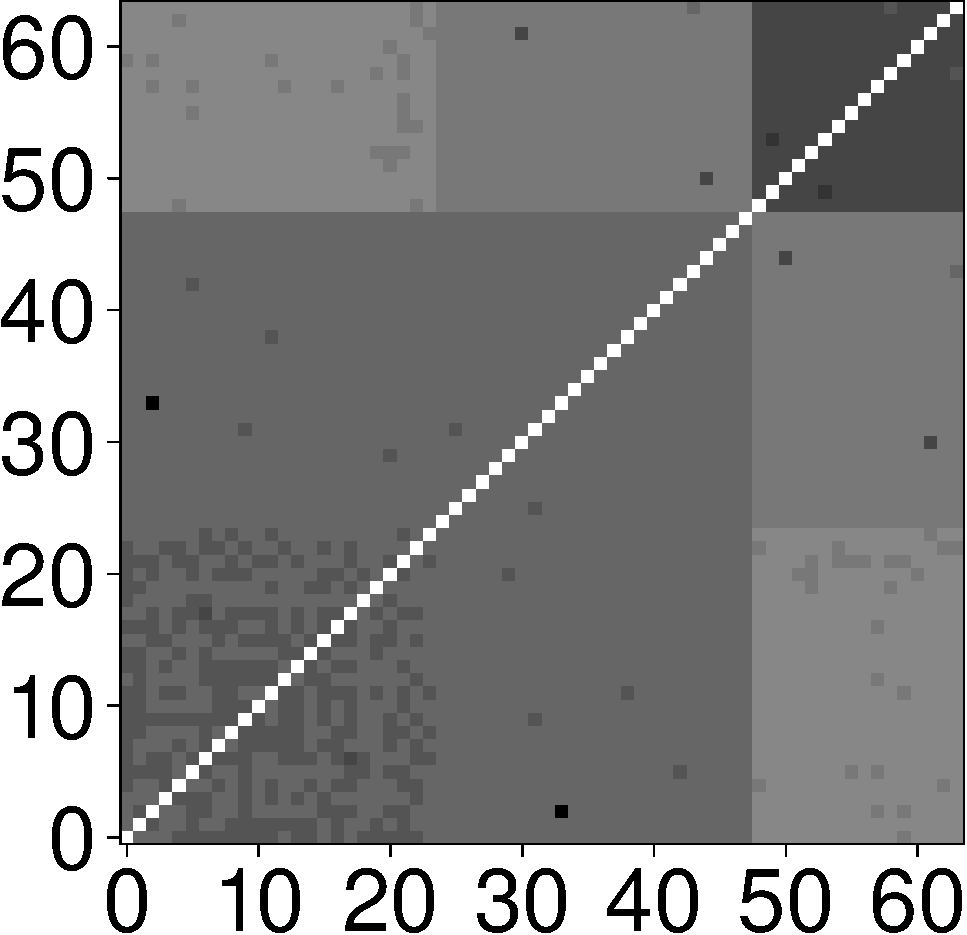
\includegraphics[width=\oneFPage\textwidth]{figures/mechanism/matrices/xeon/ssca2_64.pdf}
	}
	\subfigure[vacation]{
		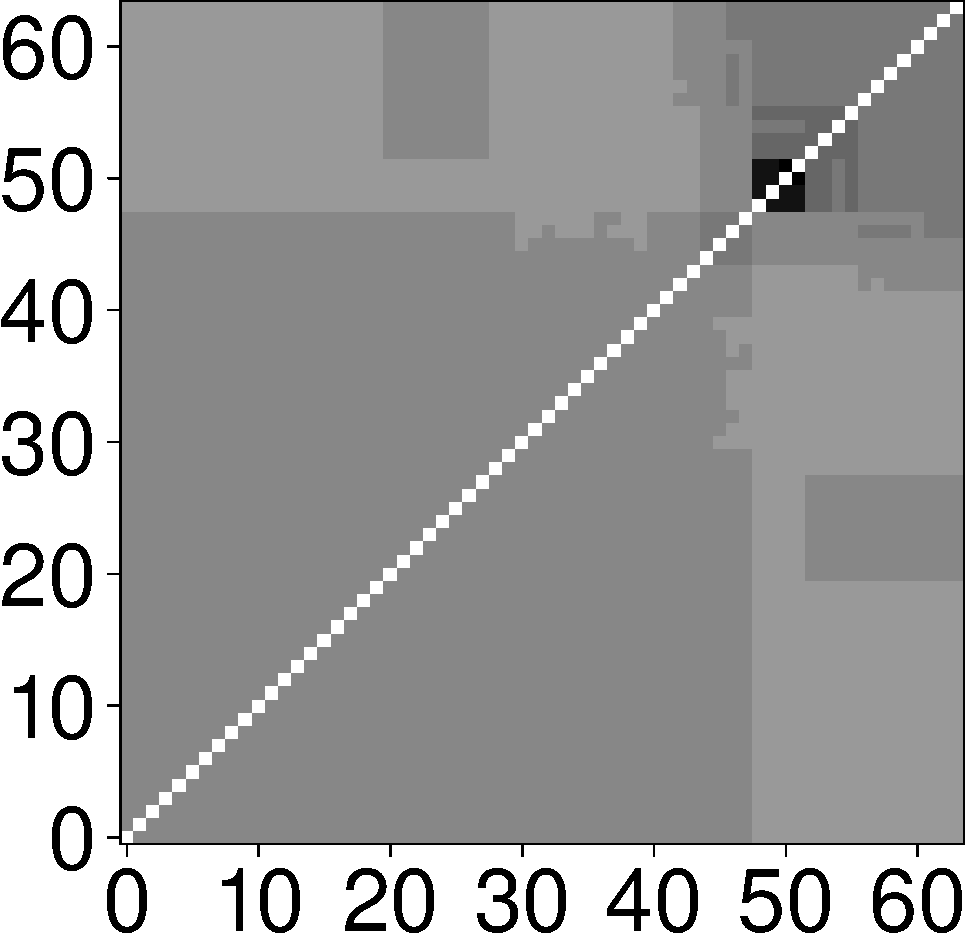
\includegraphics[width=\oneFPage\textwidth]{figures/mechanism/matrices/xeon/vacation_64.pdf}
	}
	\subfigure[yada]{
		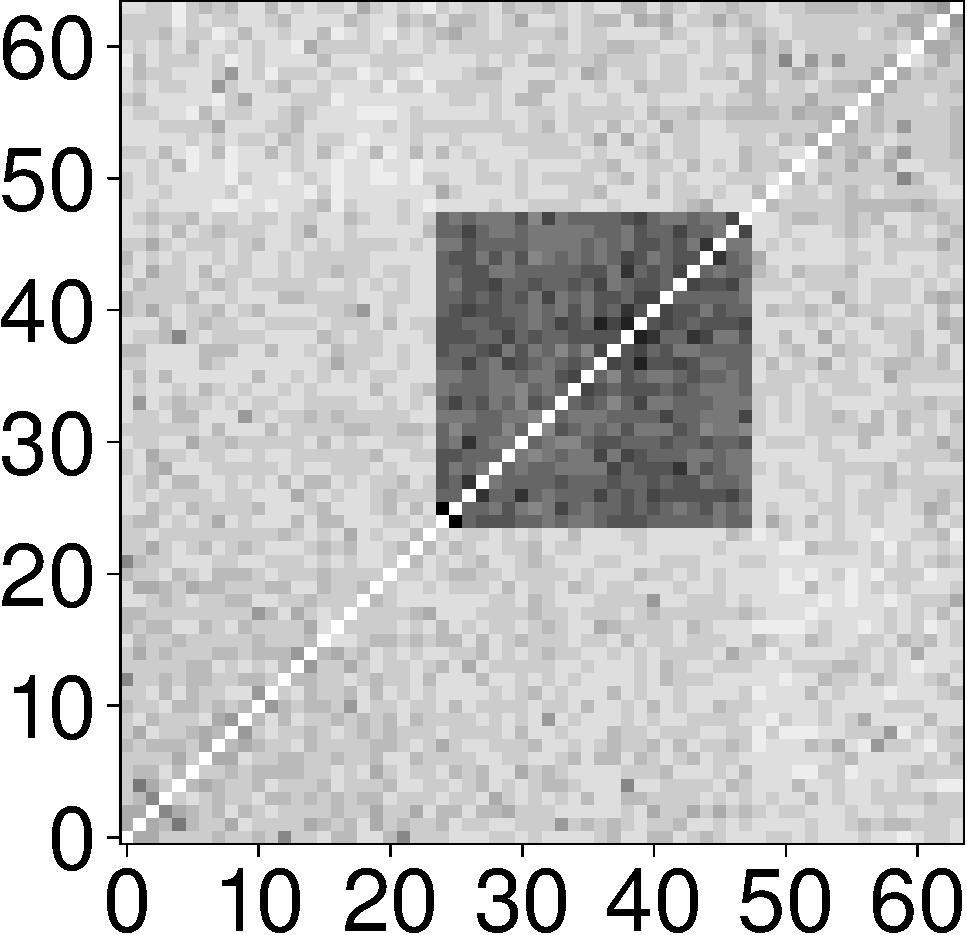
\includegraphics[width=\oneFPage\textwidth]{figures/mechanism/matrices/xeon/yada_64.pdf}
	}
	\subfigure[redblacktree]{
		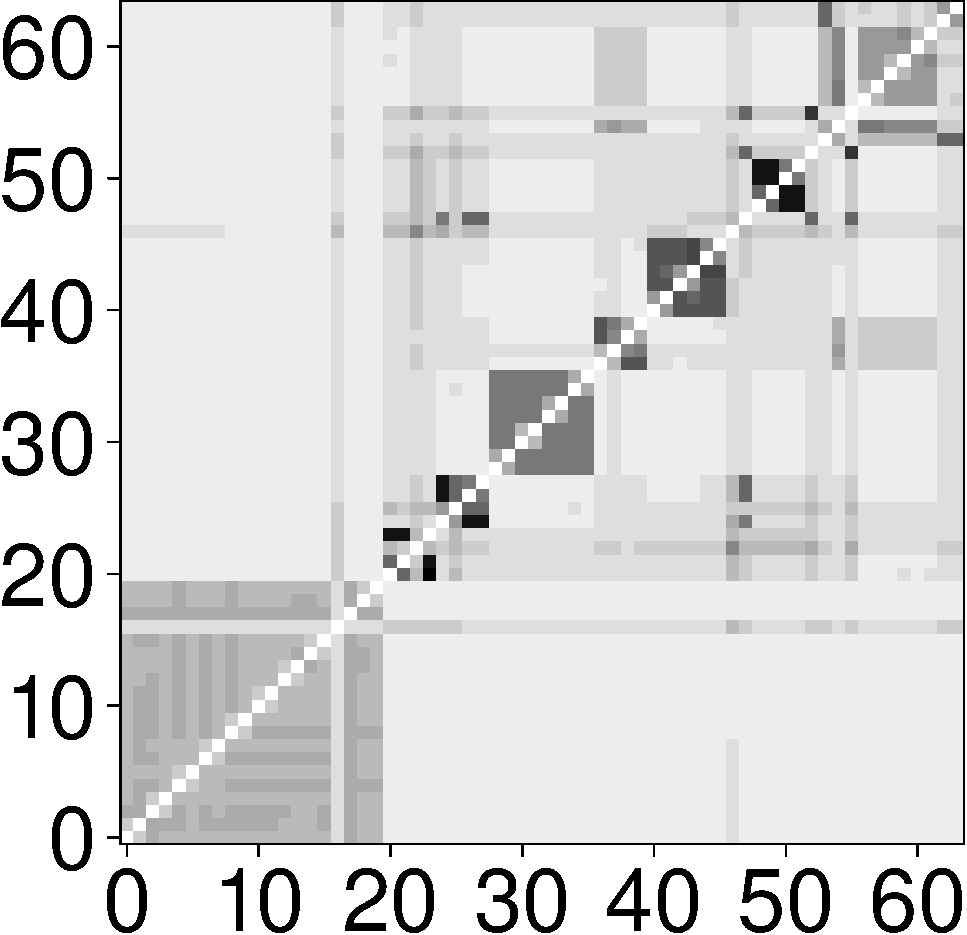
\includegraphics[width=\oneFPage\textwidth]{figures/mechanism/matrices/xeon/redblacktree_64.pdf}
	}
	\subfigure[hashmap]{
		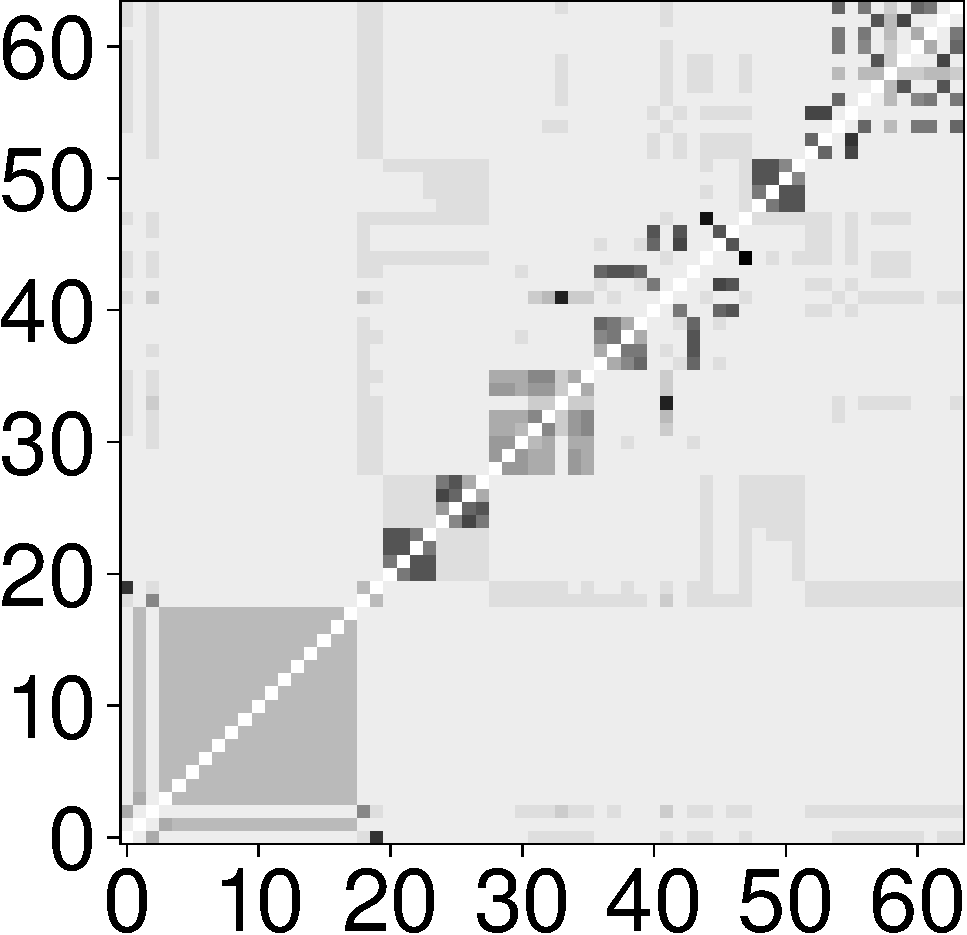
\includegraphics[width=\oneFPage\textwidth]{figures/mechanism/matrices/xeon/hashmap_64.pdf}
	}
	\caption{Communication matrices - 64 threads.}
\end{figure}

\begin{figure}[!tb]
	\centering
	\subfigure[bayes]{
		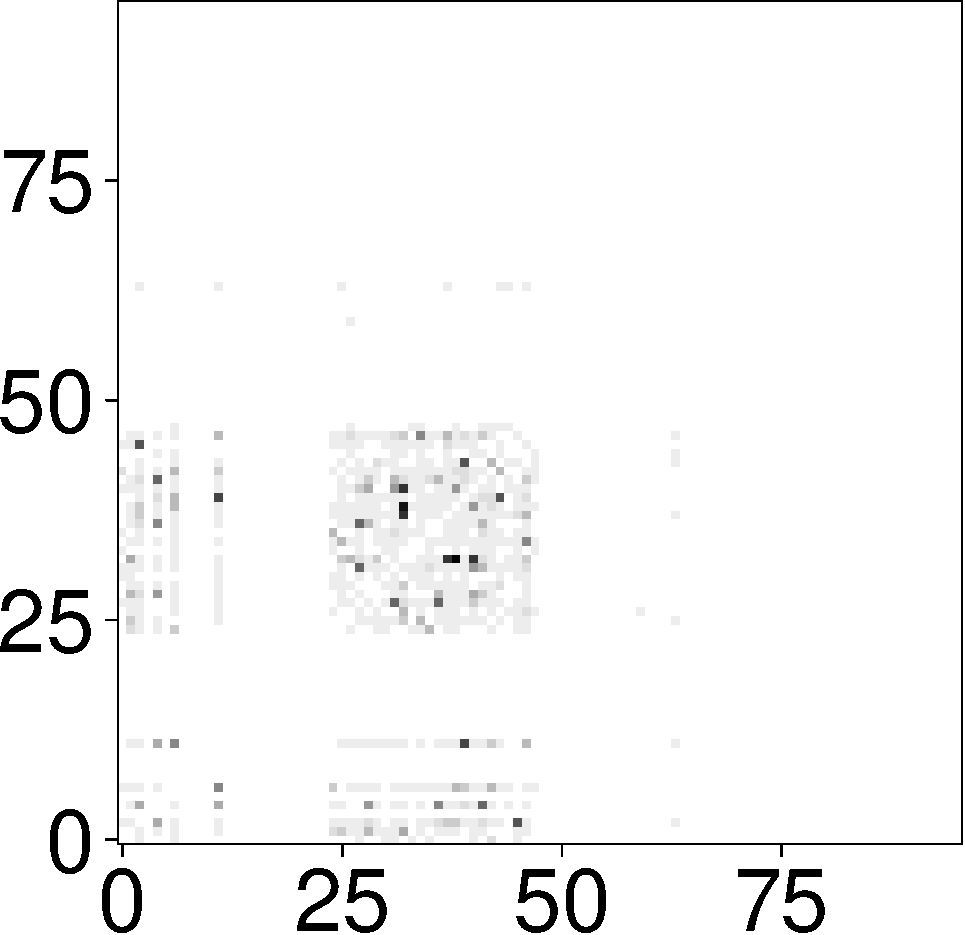
\includegraphics[width=\oneFPage\textwidth]{figures/mechanism/matrices/xeon/bayes_96.pdf}
	}
	\subfigure[genome]{
		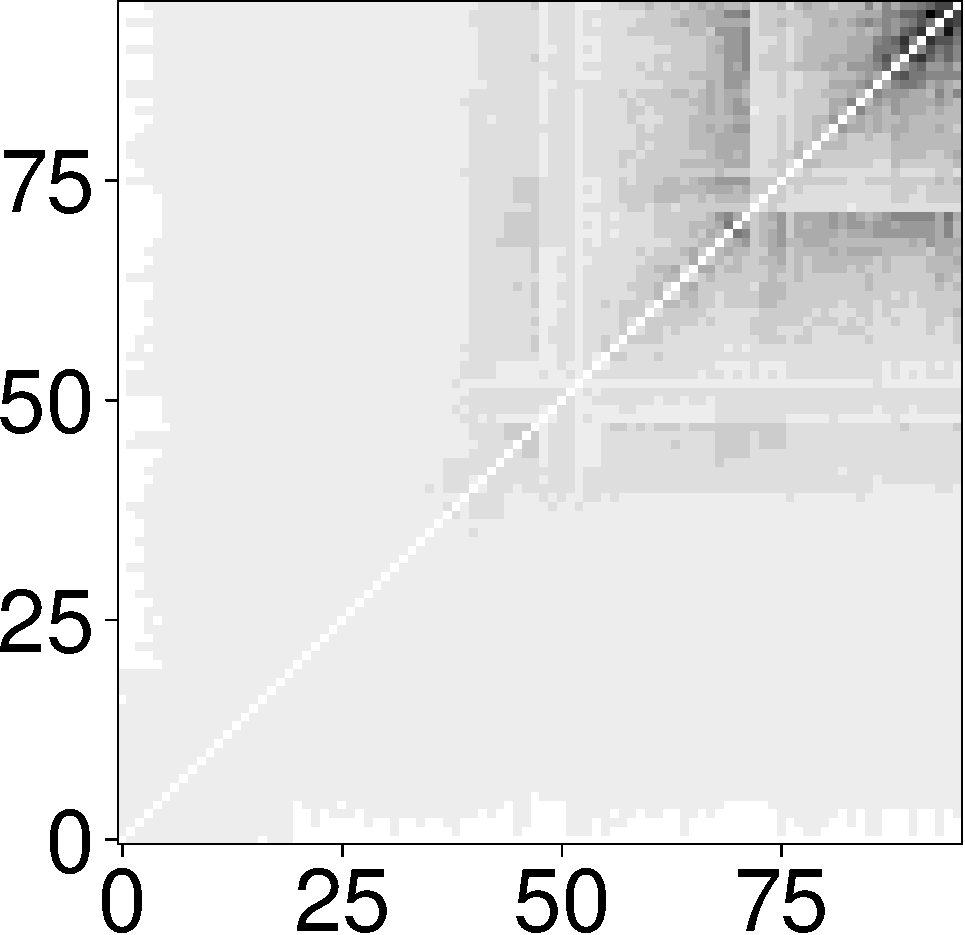
\includegraphics[width=\oneFPage\textwidth]{figures/mechanism/matrices/xeon/genome_96.pdf}
	}
	\subfigure[intruder]{
		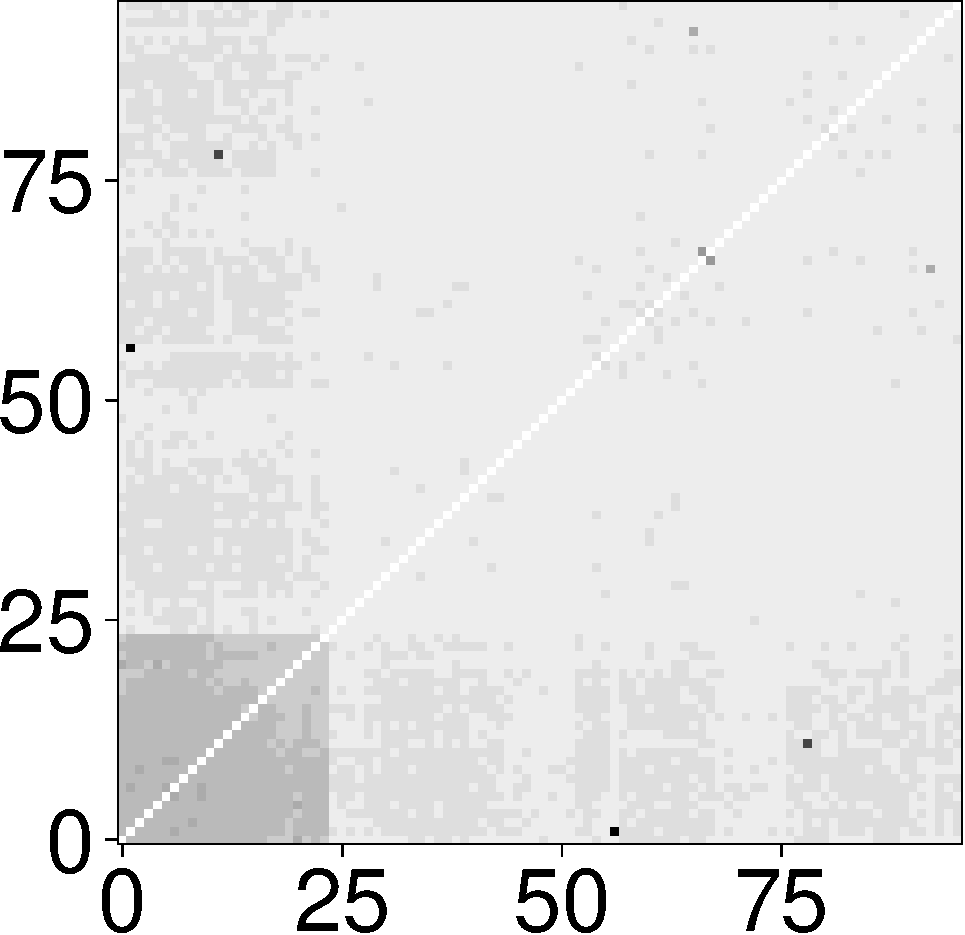
\includegraphics[width=\oneFPage\textwidth]{figures/mechanism/matrices/xeon/intruder_96.pdf}
	}
	\subfigure[kmeans]{
		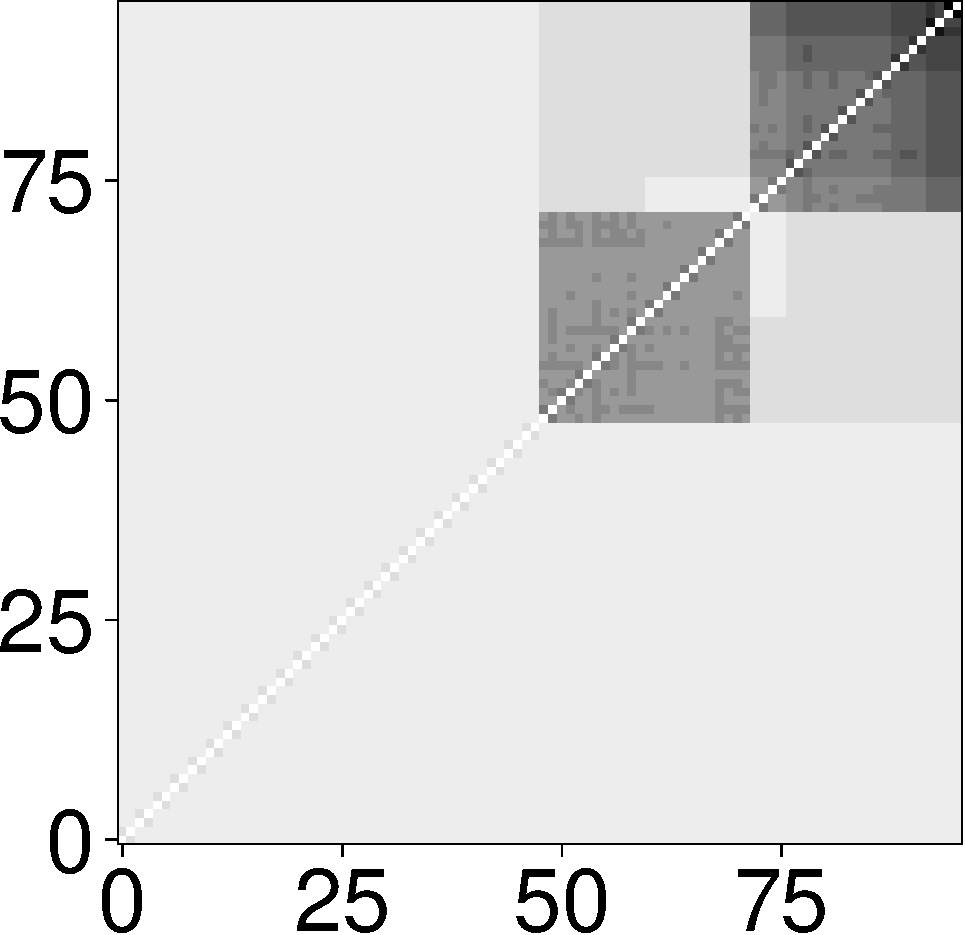
\includegraphics[width=\oneFPage\textwidth]{figures/mechanism/matrices/xeon/kmeans_96.pdf}
	}
	\subfigure[labyrinth]{
		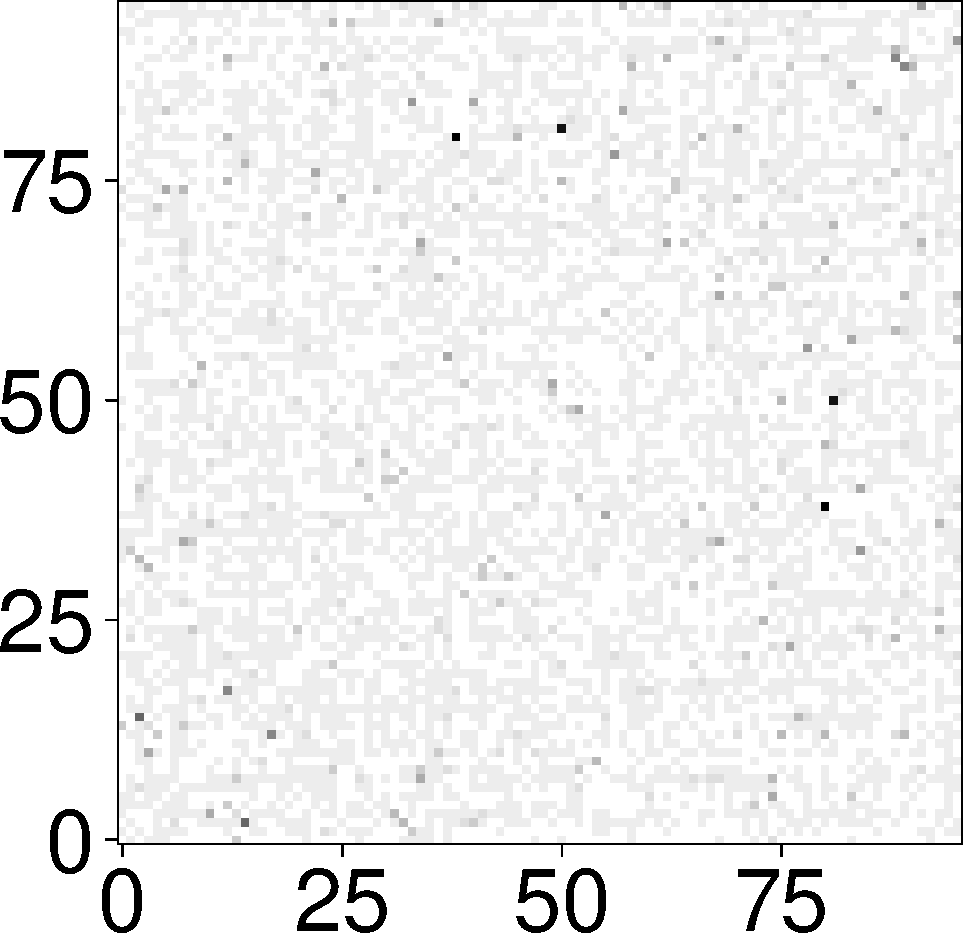
\includegraphics[width=\oneFPage\textwidth]{figures/mechanism/matrices/xeon/labyrinth_96.pdf}
	}
	\\
	\subfigure[ssca2]{
		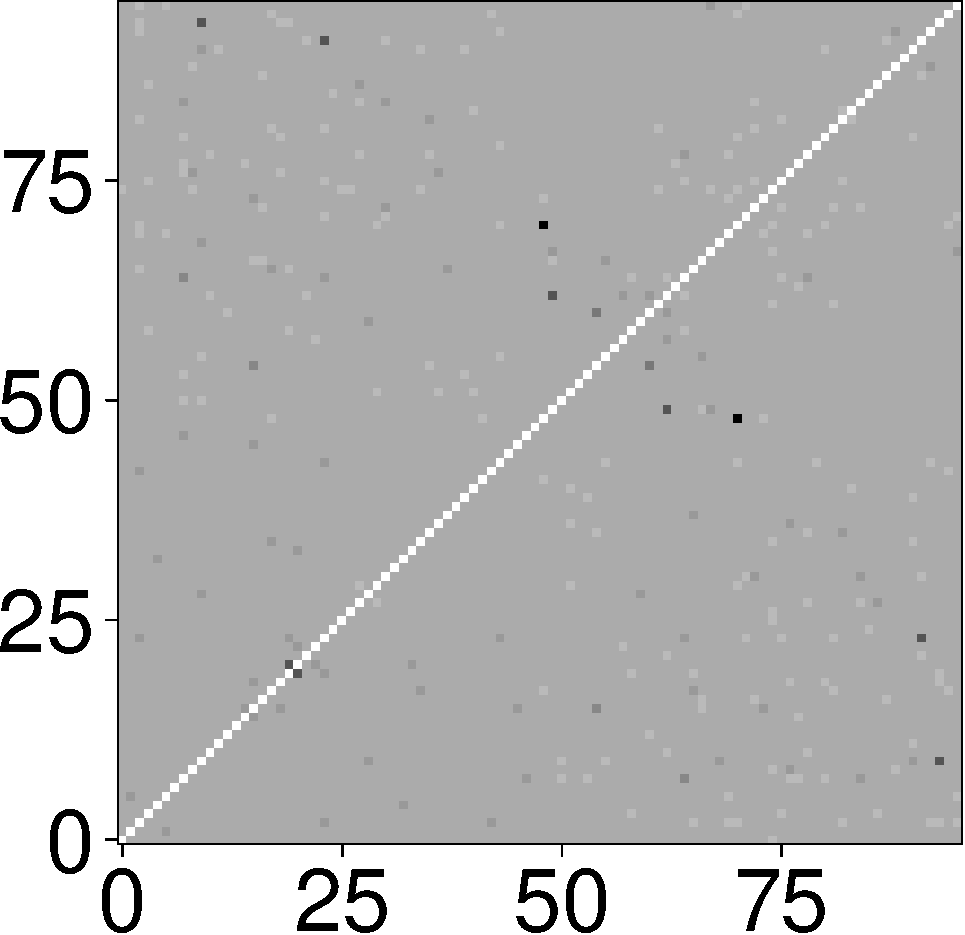
\includegraphics[width=\oneFPage\textwidth]{figures/mechanism/matrices/xeon/ssca2_96.pdf}
	}
	\subfigure[vacation]{
		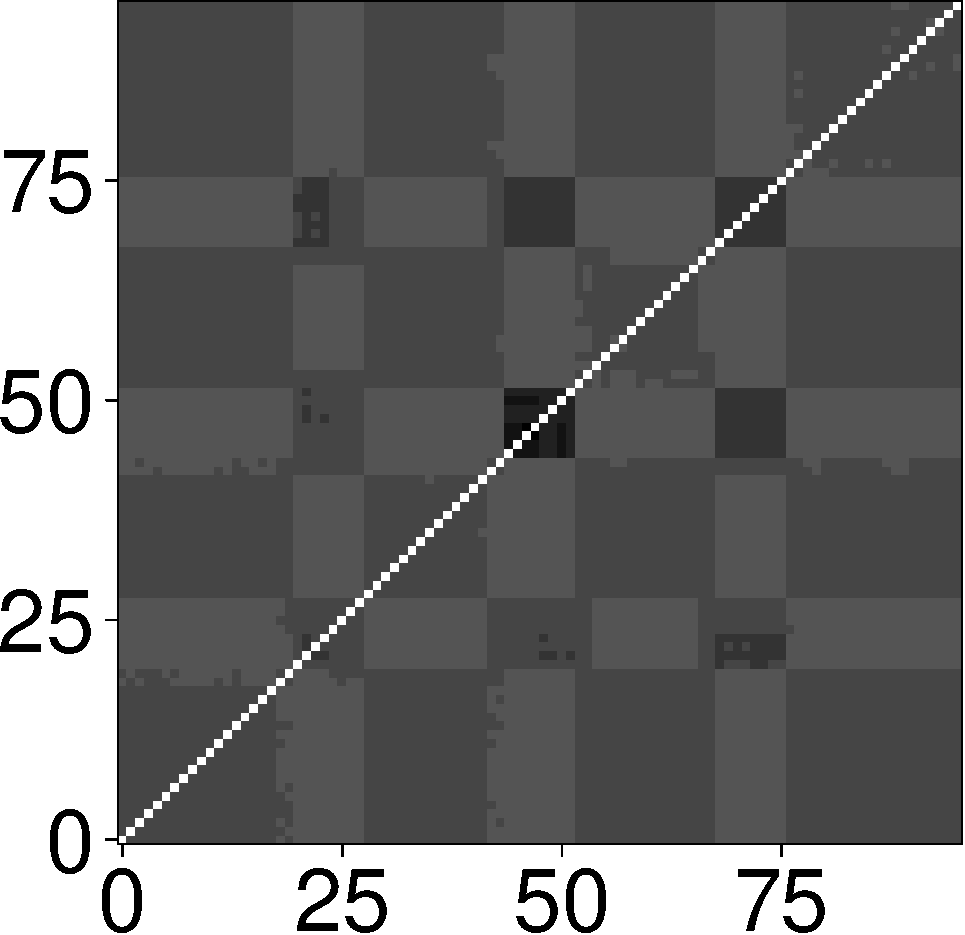
\includegraphics[width=\oneFPage\textwidth]{figures/mechanism/matrices/xeon/vacation_96.pdf}
	}
	\subfigure[yada]{
		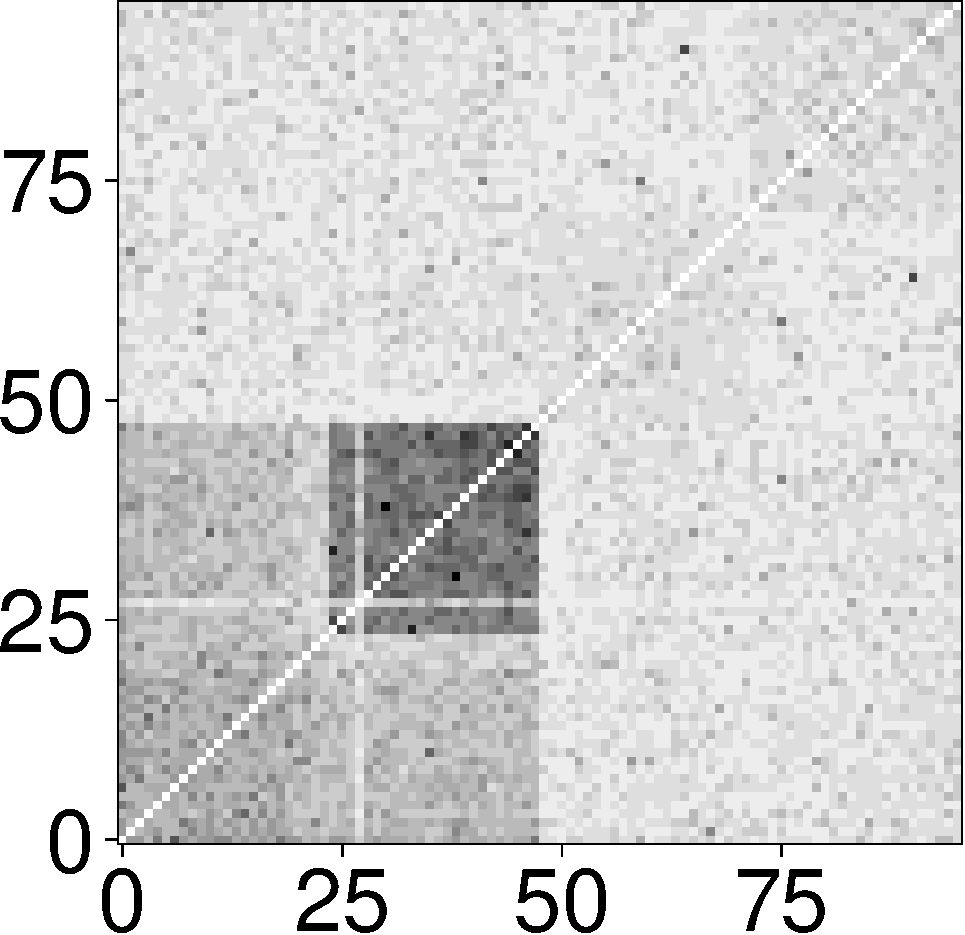
\includegraphics[width=\oneFPage\textwidth]{figures/mechanism/matrices/xeon/yada_96.pdf}
	}
	\subfigure[redblacktree]{
		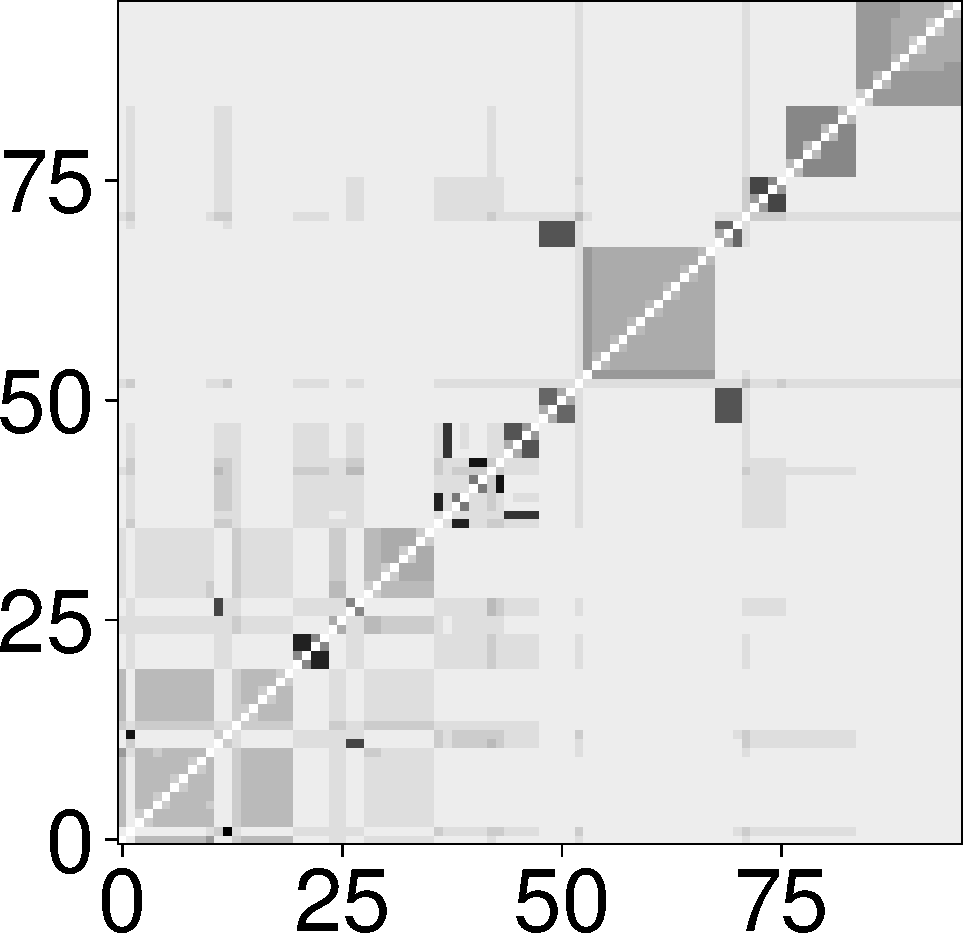
\includegraphics[width=\oneFPage\textwidth]{figures/mechanism/matrices/xeon/redblacktree_96.pdf}
	}
	\subfigure[hashmap]{
		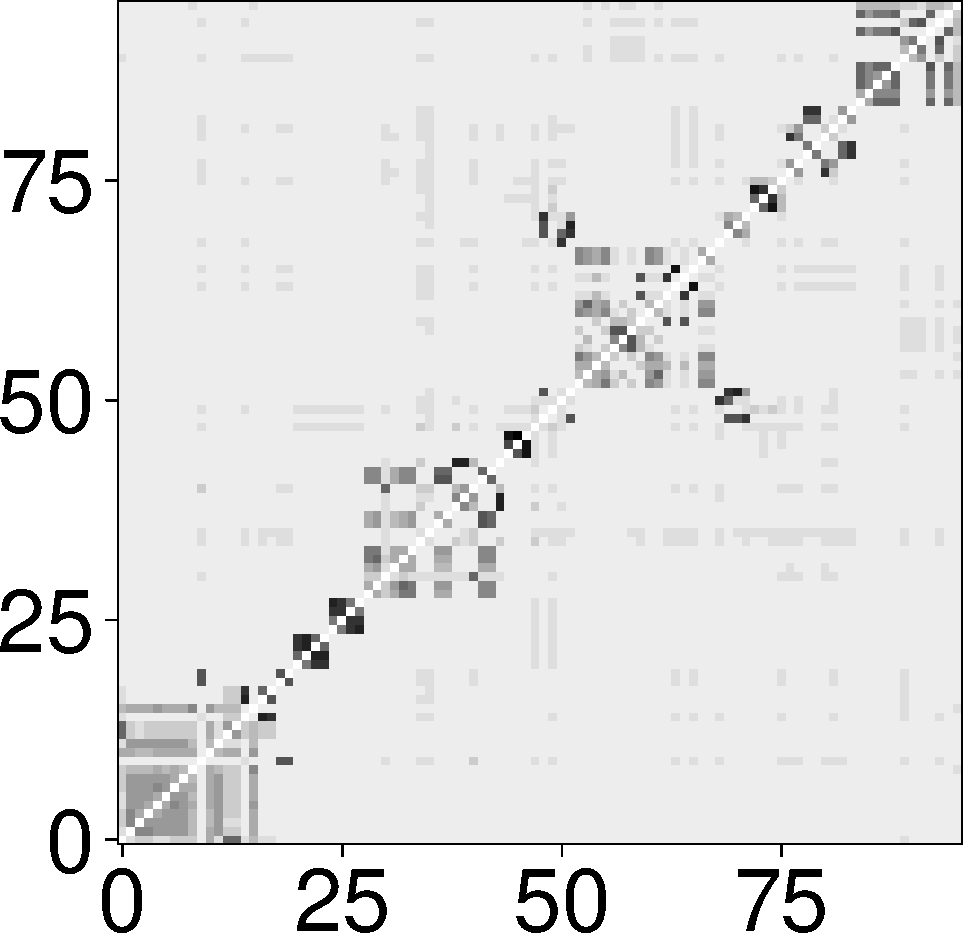
\includegraphics[width=\oneFPage\textwidth]{figures/mechanism/matrices/xeon/hashmap_96.pdf}
	}
	\caption{Communication matrices - 96 threads.}
	\label{fig:commMatrXeon96}
\end{figure}

